%==================================================================================================
\chapter{Acoplamento fluido-estrutura} \label{AFE}
%==================================================================================================

Para se descrever o problema acoplado, seja $\Omega_F$ o domínio do fluido, $\Omega_S$ o domínio da estrutura, $\Omega_\mathrm{IFE}=\Omega_F\cup\Omega_S$ o domínio do problema de IFE e $\Gamma_\mathrm{IFE}=\Omega_F\cap\Omega_S$ a interface de fluido/estrutura, conforme ilustrado na Figura \ref{fig:DomComp}.

\begin{figure}[h!]
    \centering
    \caption{Domínio computacional do problema de IFE.}
    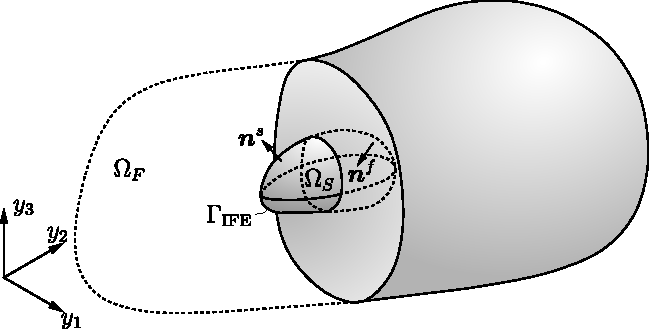
\includegraphics[width=.65\linewidth]{Figuras/Dom_Comp.pdf}
    \\Fonte: Presente trabalho (\the\year).
    \label{fig:DomComp}
\end{figure}

\citeonline{richter2017fluid} apontam três condições que devem ser satisfeitas no acoplamento: a Condição Cinemática, que diz respeito à movimentação dos domínios analisados, devendo ser compatíveis em $\Gamma_\mathrm{IFE}$, ou seja, a componente normal ao movimento deve ser igual em ambos os meios, assim como a componente tangencial em caso de condição de aderência do fluido à estrutura; a Condição Dinâmica, que aponta a continuidade das forças internas, observadas no tensor de tensões de Cauchy; e a Condição Geométrica, que exige a necessidade de ambos os domínios coincidirem em $\Gamma_\mathrm{IFE}$, não havendo sobreposições nem formação de vazios.

Numericamente, há diversas possibilidades para que essas condições sejam impostas de forma exata ou aproximada, sendo possível acoplamento monolítico ou acoplamento particionado, com o último ainda subdividido em particionado fraco e forte, como mencionado em \ref{IFE}.

Nas formulações adotadas para CFD e CSD, é comumente empregado o Método de Newton-Raphson para o cálculo das variáveis incógnitas. O mesmo pode ser aplicado quando do acoplamento direto, monolítico, entre os dois meios. Para isso a matriz tangente ($\BB{H}$) pode ser obtida por \cite{bazilevs2013computational,sanches2022metodos}:

\begin{equation}
    \BB{H}=\frac{\partial^2\script{G}}{\partial\BB{\Psi}\otimes\partial\DOF}\text{,}
\end{equation}

\noindent sendo $\script{G}$ a soma de todas as equações diferenciais do problema em sua forma fraca, $\BB{\Psi}$ o vetor com todos os parâmetros nodais das funções teste e $\DOF$ o vetor com todos os parâmetros nodais incógnitas do problema. Assim, obtém-se a correção dos valores das variáveis por meio da solução do sistema:

\begin{equation}
    \BB{H}\Delta\DOF=-\res\text{,}
\end{equation}

\noindent em que $\res=\partial\script{G}/\partial\BB{\Psi}$ é o vetor resíduo.

Expandindo a matriz em submatrizes a fim de visualizar a contribuição de cada parcela no sistema global tem-se:

\begin{equation}
    \begin{bmatrix}
        \BB{H}_{11} & \BB{H}_{12} & \BB{H}_{13} \\
        \BB{H}_{21} & \BB{H}_{22} & \BB{H}_{23} \\
        \BB{H}_{31} & \BB{H}_{32} & \BB{H}_{33}
    \end{bmatrix}\begin{bmatrix}
        \Delta\DOF_1 \\\Delta\DOF_2\\\Delta\DOF_3
    \end{bmatrix}=-\begin{bmatrix}
        \res_1 \\\res_2\\\res_3
    \end{bmatrix}\text{,}
\end{equation}

\noindent sendo os subíndices $1$, $2$ e $3$ referentes às variáveis do fluido, da estrutura e da malha, respectivamente.

Já o acoplamento particionado trata o sistema de forma a eliminar os termos cruzados da matriz tangente, resultando em blocos de sistema que podem ser resolvidos independentemente \cite{bazilevs2013computational}:

\begin{equation}
    \begin{bmatrix}
        \BB{H}_{11} & \BB{0}      & \BB{0}      \\
        \BB{0}      & \BB{H}_{22} & \BB{0}      \\
        \BB{0}      & \BB{0}      & \BB{H}_{33}
    \end{bmatrix}\begin{bmatrix}
        \Delta\DOF_1 \\\Delta\DOF_2\\\Delta\DOF_3
    \end{bmatrix}=-\begin{bmatrix}
        \res_1 \\\res_2\\\res_3
    \end{bmatrix}\text{.}
\end{equation}

Note que o método continua sendo consistente, uma vez que apenas a matriz tangente do método de Newton-Raphson foi modificada, no entanto, a convergência não é garantida.
Para aprimorar os resultados, em cada iteração $k$ do processo de Newton-Raphson, pode-se resolver sequencialmente os blocos e atualizar os valores calculados em um bloco para o cálculo do próximo, sendo obtido pelo procedimento apresentado no Algoritmo \ref{alg:acoplamentoForte}, tornando o processo de solução análogo ao método de Gauss-Seidel. Essa forma de acoplamento é denominada acoplamento particionado forte, onde, havendo convergência, a mesma resposta do acoplamento monolítico deve ser alcançada.

\begin{algorithm}[h!]
    \caption{Processo de acoplamento particionado forte}
    \label{alg:acoplamentoForte}
    \ForEach{\textnormal{passo de tempo}}{
        Atualizar valores passados do fluido, sólido e malha\;
        \ForEach{\textnormal{iteração $k$ de Newton-Raphson}}{
            \textbf{Resolver fluido}: $\BB{H}_{11}^k(\DOF_1^k,\DOF_2^k,\DOF_3^k)\Delta\DOF_1^k=-\res_1^k(\DOF_1^k,\DOF_2^k,\DOF_3^k)$\\
            Atualizar valores atuais do fluido: $\DOF_1^{k+1}\gets\DOF_1^k+\Delta\DOF_1^k$\\
            Atualizar forças de superfície no sólido: $\BB{t}^s=-\BB{\sigma}^f\cdot\BB{n}^f$\\
            Calcular medida de convergência $\epsilon_f$\;
            \textbf{Resolver sólido}: $\BB{H}_{22}^k(\DOF_1^{k+1},\DOF_2^k,\DOF_3^k)\Delta\DOF_2^k=-\res_2^k(\DOF_1^{k+1},\DOF_2^k,\DOF_3^k)$\\
            Atualizar valores atuais do sólido:  $\DOF_2^{k+1}\gets\DOF_2^k+\Delta\DOF_2^k$\\
            Atualizar velocidades e acelerações do fluido em $\Gamma_\mathrm{IFE}$;\\
            Atualizar deslocamentos e acelerações na malha em $\Gamma_\mathrm{IFE}$;\\
            Calcular medida de convergência $\epsilon_s$\;
            \textbf{Resolver malha}: $\BB{H}_{33}^k(\DOF_1^{k+1},\DOF_2^{k+1},\DOF_3^k)\Delta\DOF_3^k=-\res_3^k(\DOF_1^{k+1},\DOF_2^{k+1},\DOF_3^k)$\\
            Atualizar valores atuais da malha: $\DOF_3^{k+1}\gets\DOF_3^k+\Delta\DOF_3^k$\\
            Calcular medida de convergência $\epsilon_m$\;
            \lIf{$\epsilon_f<\mathrm{tol}_f$, $\epsilon_s<\mathrm{tol}_s$ e $\epsilon_m<\mathrm{tol}_m$}{Sair do \textit{loop}}
        }
    }
\end{algorithm}

Caso os blocos sejam resolvidos em processos iterativos separados, sem que haja atualização das variáveis de um problema para o outro dentro de cada processo iterativo, fazendo a atualização apenas ao final de cada passo no tempo, tem-se um modelo de acoplamento denominado acoplamento particionado fraco. Para construir um acoplamento particionado fraco, pode-se assumir que o problema do fluido depende das variáveis do sólido e da malha em um instante $t$ e das variáveis do fluido em um instante $t+1$, já o problema do sólido depende do valor das variáveis do fluido e do sólido em um tempo $t+1$ e, por fim, o problema da malha depende das variáveis do sólido e da malha em um instante $t+1$. Assim, o cálculo é realizado segundo o Algoritmo \ref{alg:PartFraco}, no qual $k_f$, $k_s$ e $k_m$ são as iterações das soluções dos problemas de fluido, estrutura e malha, respectivamente \cite{sanches2022metodos}. Ainda é observado que a movimentação da malha segue um problema linear, sendo seu resultado obtido diretamente em uma iteração.

\begin{algorithm}[h!]
    \caption{Processo de acoplamento particionado fraco}
    \label{alg:PartFraco}

    \ForEach{\textnormal{passo de tempo}}{
    Atualizar valores passados do fluido, sólido e malha\;
    \ForEach{\textnormal{iteração $k_f$ de Newton-Raphson}}{
    \textbf{Resolver fluido}: $\BB{H}_{11}((\DOF_1^{k_f})^{t+1},(\DOF_2)^t,(\DOF_3)^t)\Delta(\DOF_1^{k_f})^{t+1}=-\res_1((\DOF_1^{k_f})^{t+1},(\DOF_2)^t,(\DOF_3)^t)$\;
    Atualizar valores: $(\DOF_1^{k_f+1})^{t+1}\gets(\DOF_1^{k_f})^{t+1}+\Delta(\DOF_1^{k_f})^{t+1}$\;
    % Calcular medida de convergência $\epsilon_f$\;
    \lIf{$\epsilon_f<\mathrm{tol}_f$}{Sair do \textit{loop}}
    }
    Atualizar forças de superfície no sólido: $\BB{t}^s=-\BB{\sigma}^f\cdot\BB{n}^f$\\
    \ForEach{\textnormal{iteração $k_s$ de Newton-Raphson}}{
    \textbf{Resolver sólido}: $\BB{H}_{22}((\DOF_1)^{t+1},(\DOF_2^{k_s})^{t+1})\Delta(\DOF_2^{k_s})^{t+1}=-\res_2((\DOF_1)^{t+1},(\DOF_2^{k_s})^t)$\;
    Atualizar valores: $(\DOF_2^{k_s+1})^{t+1}\gets(\DOF_2^{k_s})^{t+1}+\Delta(\DOF_2^{k_s})^{t+1}$\;
    % Calcular medida de convergência $\epsilon_s$\;
    \lIf{$\epsilon_s<\mathrm{tol}_s$}{Sair do \textit{loop}}
    }
    Atualizar velocidades e acelerações do fluido em $\Gamma_\mathrm{IFE}$;\\
    Atualizar deslocamentos e acelerações na malha em $\Gamma_\mathrm{IFE}$;\\
    \ForEach{\textnormal{iteração $k_m$ de Newton-Raphson}}{
    \textbf{Resolver malha}: $\BB{H}_{3}((\DOF_3^{k_m})^{t+1},(\DOF_2)^t)\Delta(\DOF_3^{k_s})^{t+1}=-\res_3((\DOF_3^{k_m})^{t+1},(\DOF_2)^t)$\;
    Atualizar valores: $(\DOF_3^{k_m+1})^{t+1}\gets(\DOF_3^{k_m})^{t+1}+\Delta(\DOF_3^{k_m})^{t+1}$\;
    % Calcular medida de convergência $\epsilon_m$\;
    \lIf{$\epsilon_m<\mathrm{tol}_m$}{Sair do \textit{loop}}
    }
    }
\end{algorithm}

Por dispensar etapas de correção, esse método possui um custo computacional menor em relação ao particionado forte, no entanto exige a adoção de passos de tempo pequenos e fica sujeito a problemas de instabilidades como mencionado em \citeonline{Felippaetal2001}. Nota-se que esse tipo de acoplamento é mais adequado a problemas com escoamento compressível, onde um passo de tempo pequeno é necessário para se capturar a propagação de ondas de choque ao mesmo tempo em que a massa específica do fluido costuma ser muito menor que a do sólido.

Por outro lado, a convergência do processo de acoplamento particionado forte pode ficar prejudicada, especialmente à medida em que a massa específica do fluido e do sólido se aproximam, ou em outros problemas fortemente acoplados, onde uma pequena perturbação do fluido pode produzir grandes perturbações na estrutura e vice-versa. Como meios de garantir convergência nessa situação, mantendo o acoplamento particionado, pode-se adotar relaxações de Aitken, destinadas melhorar a convergência no método de Gauss-Seidel, na atualização das variáveis \cite{fernandes2019ale} ou aplicar um fator de escala sobre a matriz de massa do sólido (técnica \textit{Augmented $A_{22}$}) \cite{tezduyar2005finite}. Por simplicidade, neste trabalho, em um exemplo onde foi necessário, adotou-se a segunda técnica.

%==================================================================================================
\section{Exemplos para verificação}
%==================================================================================================

Na presente as formulações implementadas são aplicadas à simulação de problemas de interação fluido-estruturas selecionados para a verificação do código computacional, bem como para o estudo das características das formulações implementadas quando aplicadas à análise de IFE.

%==================================================================================================
\subsection{Cavidade com fundo flexível} \label{FSI-Cavity2D}
%==================================================================================================

O primeiro exemplo utilizado para verificação do acoplamento IFE forte tipo bloco-iterativo, trata-se de uma cavidade semelhante à do exemplo \ref{ex:cavity}, porém com velocidade tangencial oscilatória no topo e com fundo flexível, como ilustrado na Figura \ref{fig:cavity2D}. Tal exemplo, embora seja caracterizado pelo comportamento bidimensional, é simulado aqui por discretização 3D, sendo aplicadas condições de paredes lisas nas faces paralelas ao escoamento, e condição de simetria (componente do vetor generalizado na direção 3 restrita) para a casca. Esse problema foi estudado por \citeonline{gerbeau2003quasi}, sendo que a estrutura apresenta: massa específica $\rho_S=500$, módulo de Young $E=250$, coeficiente de Poisson $\nu=0$ e espessura $h=0,002$. Já o fluido apresenta: massa específica $\rho_F=1$ e viscosidade dinâmica $\mu=0,01$. A velocidade variável ao longo do tempo, imposta na direção horizontal da face superior, é dada por $u_1(t)=1-\cos{(0,4\pi t)}$, de forma que, tomando-se o comprimento característico o tamanho do lado da cavidade, o número de Reynolds varia dinamicamente de 0 a 200.

\begin{figure}[h!]
    \centering
    \caption{Cavidade com fundo flexível.}
    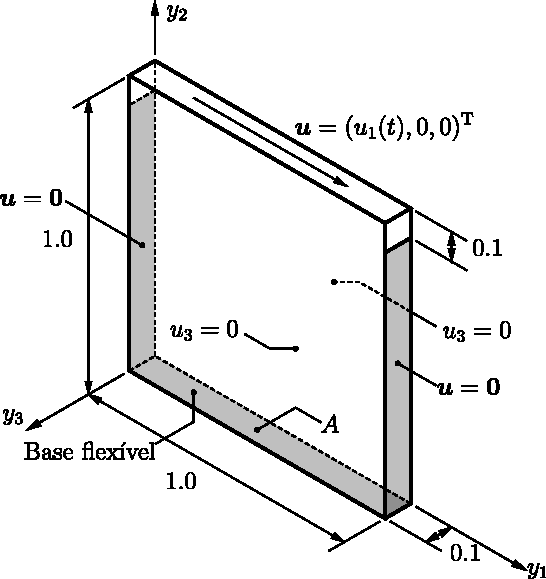
\includegraphics[width=0.5\linewidth]{Figuras/FSI-Cavity2D/FSI-Cavity2D.pdf}
    \\Fonte: Presente trabalho (\the\year).
    \label{fig:cavity2D}
\end{figure}

Considerou-se o intervalo total $t\in[0,60]$ para a simulação, discretizado em passos $\Delta t=0,1$, e considerando-se $\rho_\infty=0$ A escolha por $\rho_\infty=0$ foi feita buscando-se melhor estabilidade, uma vez que, de acordo com o relato de \citeonline{forster2007artificial}, integradores temporais de segunda ordem clássicos levaram a instabilidades imediatas. No entanto, dadas as diferenças nas formulações, não se pode descartar que outros valores de raio espectral possam conduzir a resultados estáveis e precisos.

Uma primeira simulação é conduzida apenas para verificar o acoplamento fluido-estrutura, não sendo considerados os modelos VMS nem LES. São consideradas as seguintes combinações de discretização espacial e formulação numérica: 1) malha com 1957 elementos tetraédricos P1P1, resultando em 707 nós e 2828 graus de liberdade com estabilização SUPG/PSPG; 2) malha com 1957 elementos P2P2, resultando em 4071 nós e 16284 graus de liberdade, com estabilização SUPG/PSPG; 3) malha com 1957 elementos P2P1, com 707 nós para interpolação do campo de pressão e 4071 nós para interpolação do campo de velocidade, resultando em 12920 graus de liberdade, sem estabilização. Nota-se que todas as malhas para o domínio do fluido são coincidentes, alterando-se apenas os nós e as funções de forma. Já o domínio computacional da casca foi discretizado da mesma maneira para todos os casos, sendo formada por 64 elementos, 165 nós, resultando em 1155 graus de liberdade. Ambas as discretizações, do sólido e do fluido, são apresentadas na Fig. \ref{fig:Cavity2D-mesh}.

\begin{figure}[h!]
    \centering
    \caption{Cavidade com fundo flexível - Discretização}
    \begin{subfigure}[b]{0.32\textwidth}
        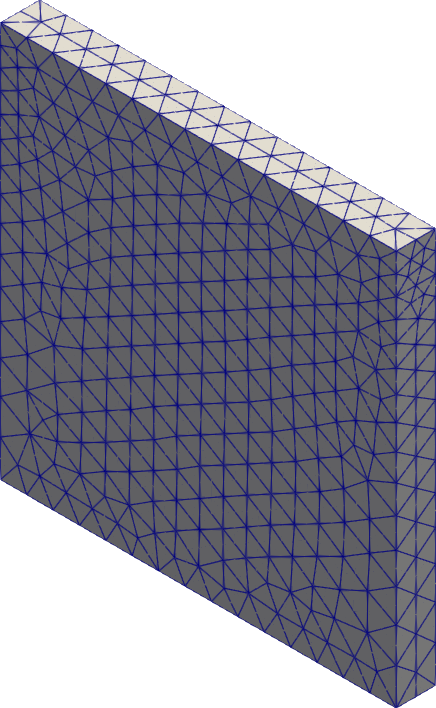
\includegraphics[width=\linewidth]{Figuras/FSI-Cavity2D/fluid-mesh.png}
        \caption{Fluido.}
    \end{subfigure}
    \begin{subfigure}[b]{0.32\textwidth}
        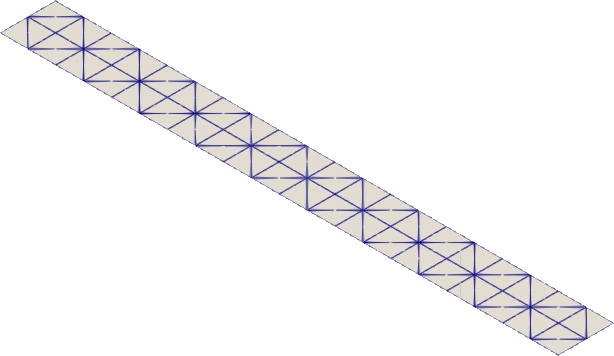
\includegraphics[width=\linewidth]{Figuras/FSI-Cavity2D/shell-mesh.png}
        \caption{Casca.}
    \end{subfigure}
    \\Fonte: Presente trabalho (\the\year).
    \label{fig:Cavity2D-mesh}
\end{figure}

Nota-se na figura \ref{fig:Cavity2D-mesh} que as malhas do estrutura e do fluido são coincidentes na interface fluido-estrutura $\Gamma_\mathrm{IFE}$, facilitando a transferência das condições de acoplamento, bem como das condições para a movimentação da malha.

Este problema mostrou-se fortemente acoplado, apresentando dificuldade de convergência para a solução bloco-iterativa. Para garantir a convergência, seguindo a técnica \textit{Augmented A22} \cite{tezduyar2005finite}, multiplicou-se a parcela da matriz tangente referente à matriz de massa da estrutura por $2,0$, o que foi suficiente para garantir boa convergência de forma consistente.

O deslocamento vertical do ponto $A$, localizado no centro da casca como ilustrado na Fig. \ref{fig:Cavity2D-mesh}, é monitorado em todas as análises, sendo a sua história apresentada na Figura \ref{fig:cavity2D-res}, onde também são comparadas com a solução obtida por \citeonline{gerbeau2003quasi}.

\begin{figure}[h!]
    \centering
    \caption{Cavidade com fundo flexível - Deslocamento vertical do nó $A$.}
    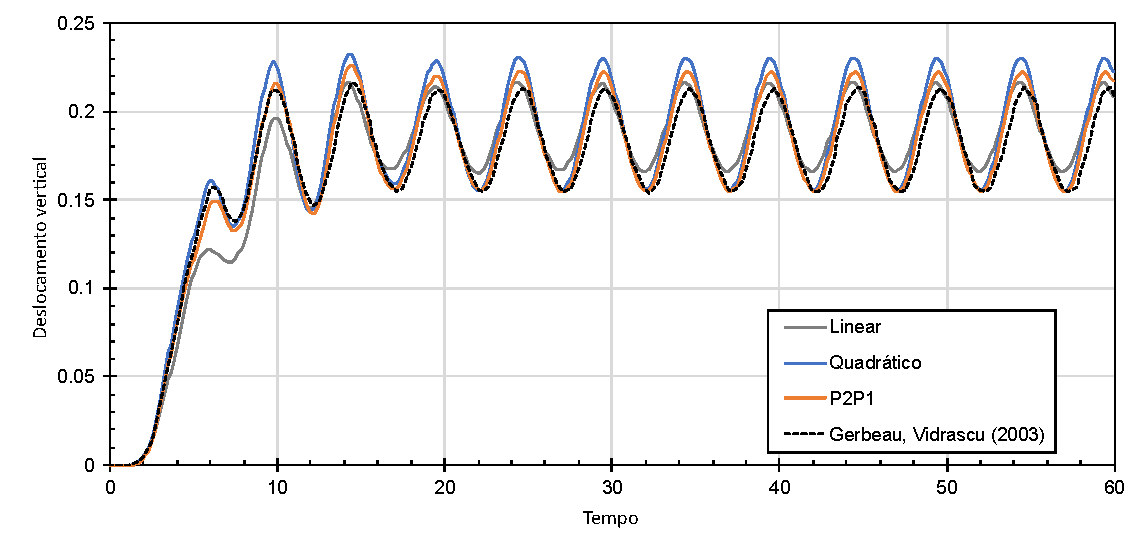
\includegraphics[width=\linewidth]{Figuras/FSI-Cavity2D/resultados.pdf}
    \\Fonte: Presente trabalho (\the\year).
    \label{fig:cavity2D-res}
\end{figure}

%\textcolor{red}{Não é empregado LES nem VMS aqui? Adote a mesma nomenclatura das simulações da cavidade rígida na legenda da figura.}

A Figura \ref{fig:cavity2D-time} apresenta o campo de pressão, assim como as linhas de corrente, para a simulação empregando-se elementos P2P2 com estabilização SUPG/PSPG nos instantes $t=3,5$, $8,0$, $14,0$ e $21,0$, os quais mostram-se qualitativamente condizentes com a solução encontrada em \citeonline{fernandes2016interaccao}.

\begin{figure}[h!]
    \centering
    \caption{Cavidade com fundo flexível - Distribuição de pressão e linhas de corrente.}
    \begin{subfigure}[b]{0.3\textwidth}
        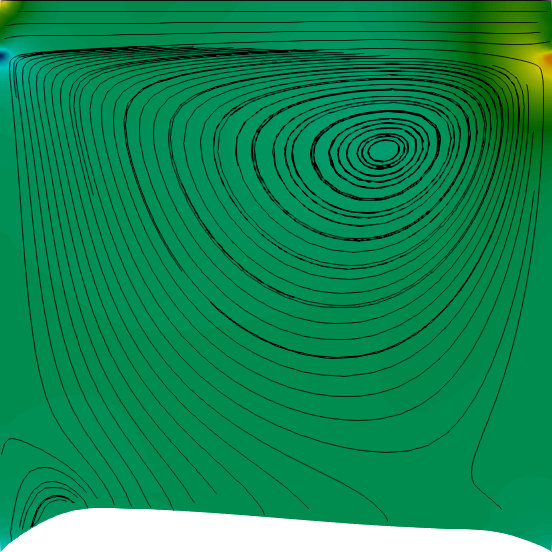
\includegraphics[width=\linewidth]{Figuras/FSI-Cavity2D/t3_5.png}
        \caption{$t=3,5$}
    \end{subfigure}
    \begin{subfigure}[b]{0.3\textwidth}
        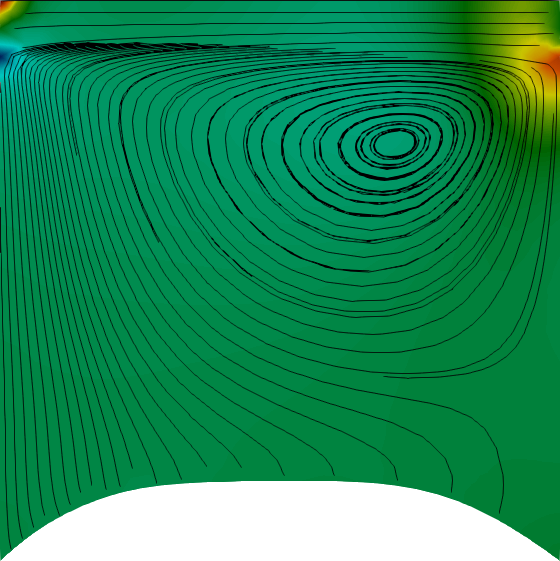
\includegraphics[width=\linewidth]{Figuras/FSI-Cavity2D/t8.png}
        \caption{$t=8,0$}
    \end{subfigure}\\
    \begin{subfigure}[b]{0.3\textwidth}
        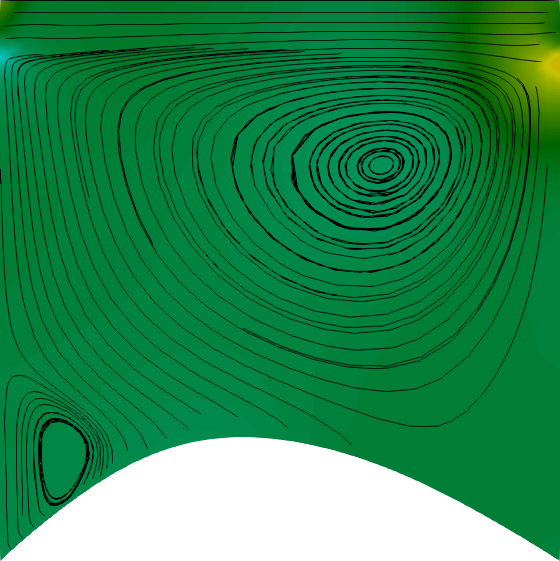
\includegraphics[width=\linewidth]{Figuras/FSI-Cavity2D/t14.png}
        \caption{$t=14,0$}
    \end{subfigure}
    \begin{subfigure}[b]{0.3\textwidth}
        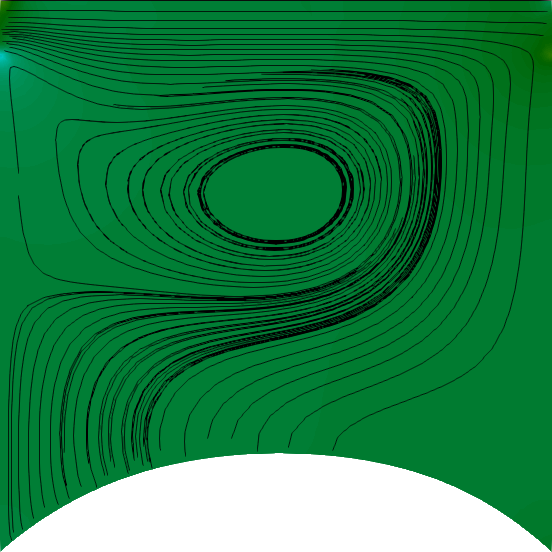
\includegraphics[width=\linewidth]{Figuras/FSI-Cavity2D/t21.png}
        \caption{$t=21,0$}
    \end{subfigure}
    \begin{subfigure}[b]{0.4\textwidth}
        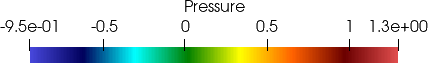
\includegraphics[width=\linewidth]{Figuras/FSI-Cavity2D/legenda.png}
    \end{subfigure}
    \\Fonte: Presente trabalho (\the\year).
    \label{fig:cavity2D-time}
\end{figure}

Esses resultados permitem evidenciar qualitativamente a consistência do acoplamento proposto.

% Visando um breve estudo qualitativo do efeito dos modelos VMS e LES, propõe-se aumentar a espessura do problema, facilitando o surgimento de estruturas tridimensionais de vorticidade. Assim, considera-se agora o domínio cúbico  realiza-se uma nova simulação considerando espessura do domínio aumentada de forma a tornar o domínio do fluido uma cavidade cúbica de lado unitário. Assim liberou-se o movimento da casca nas três direções para se obter uma melhor representatividade física. Além disso, tanto o domínio do fluido quanto o da casca foram discretizados com malhas mais pobres, com a malha do fluido possuindo 2786 elementos de aproximação quadrática, 4963 nós e 19852 graus de liberdade, enquanto a malha do sólido possui 72 elementos, 169 nós e 1183 graus de liberdade, conforme ilustrado na Fig. \ref{fig:cavity2D-coarse}.

% \begin{figure}[h!]
%     \centering
%     \caption{Cavidade com fundo flexível e domínio espesso - Discretização.}
%     \begin{subfigure}[b]{0.4\textwidth}
%         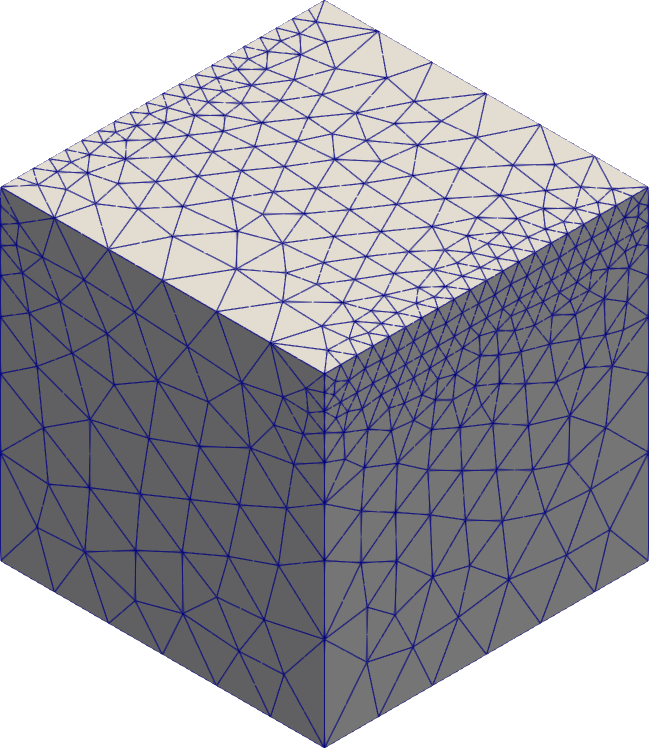
\includegraphics[width=\linewidth]{Figuras/FSI-Cavity2D/fluid-coarse.png}
%         \caption{Fluido.}
%     \end{subfigure}
%     \begin{subfigure}[b]{0.4\textwidth}
%         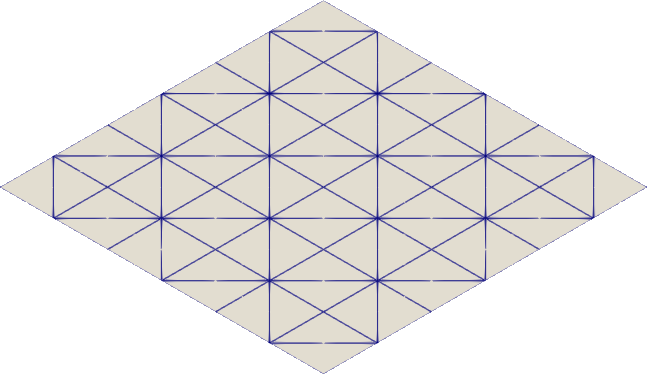
\includegraphics[width=\linewidth]{Figuras/FSI-Cavity2D/shell-coarse.png}
%         \caption{Casca.}
%     \end{subfigure}
%     \\Fonte: Presente trabalho (\the\year).
%     \label{fig:cavity2D-coarse}
% \end{figure}

% Nesse caso observou-se a influência que cada tipo de estabilização causa na solução, onde simulou-se com as estabilizações SUPG/PSPG e VMS. Também foram simulados os problemas com e sem a aplicação do modelo LES, para analisar os efeitos que este causa na solução. A Figura \ref{fig:cavity2D-rescoarse} apresenta o deslocamento vertical do centro da casca (nó $A$) ao longo do tempo, comparando-se com os resultados obtidos por \citeonline{gerbeau2003quasi}.

% \begin{figure}[h!]
%     \centering
%     \caption{Cavidade com fundo flexível e domínio espesso - Deslocamento vertical do ponto $A$.}
%     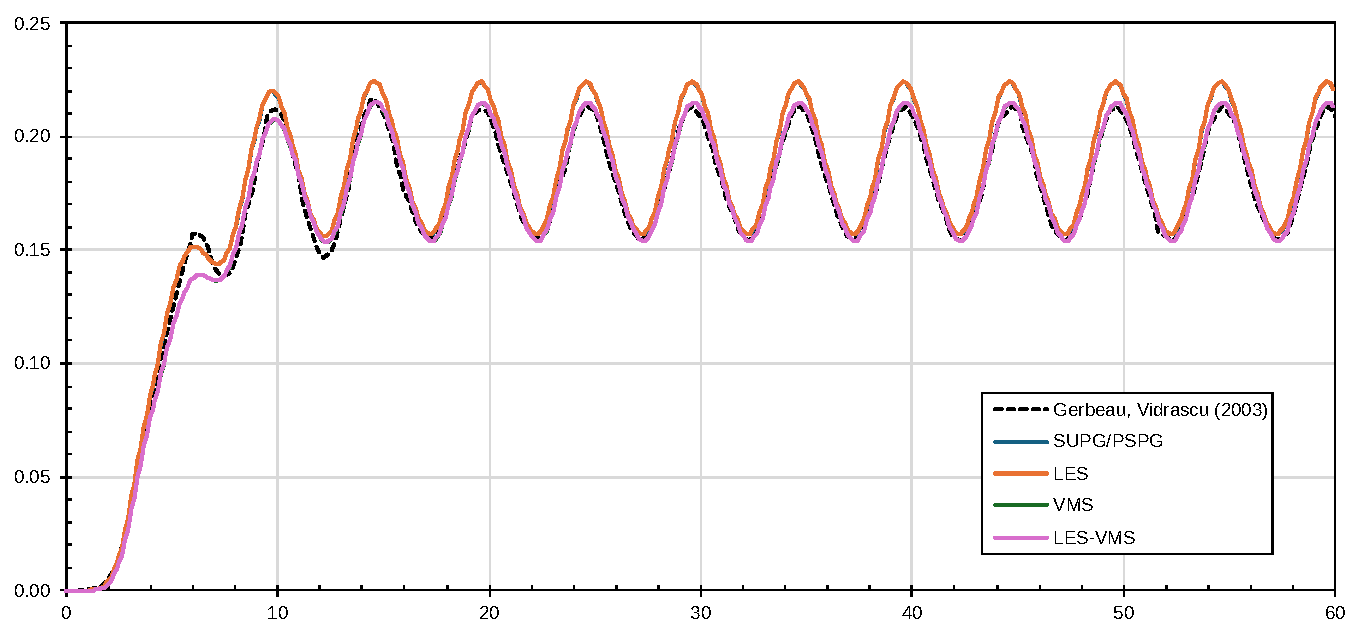
\includegraphics[width=\linewidth]{Figuras/FSI-Cavity2D/results-coarse.pdf}
%     \\Fonte: Presente trabalho (\the\year).
%     \label{fig:cavity2D-rescoarse}
% \end{figure}

% É possível perceber que a aplicação dos demais termos estabilizadores presentes na formulação VMS levaram a uma melhora na solução obtida, em relação ao SUPG/PSPG. No entanto a aplicação do modelo LES não surtiu efeito na solução encontrada. Isso se deve ao fato do número de Reynolds do problema ser baixo, além de possuir gradientes de velocidade também muito pequenos. Outro motivo que pode ter contribuído com a baixa contribuição do LES se deve ao fato do problema requerer um refinamento maior nas faces de entrada e saída do fluido, fazendo com que a face superior, como um todo, tivesse elementos menores, e é exatamente nessa região onde o LES teria seu maior impacto. Com isso, todos esses fatores somados levaram a um problema onde não se necessita a aplicação do modelo LES.

%==================================================================================================
\subsection{Cavidade tridimensional com fundo flexível}
%==================================================================================================

Este exemplo foi estudado por \citeonline{valdes2007nonlinear} e pode ser entendido como uma extensão do exemplo da exemplo \ref{FSI-Cavity2D}, em que o domínio de análise é um cubo de lado unitário cuja base é flexível. Todas as propriedades físicas, tanto do fluido quanto da casca são mantidas as mesmas. As condições de contorno no domínio do fluido também se mantém as mesmas em relação ao exemplo anterior, enquanto as condições de contorno da casca agora são de apoio nos quatro lados, ou seja, os deslocamentos em todas as direções são impedidos, enquanto as rotações (os vetores generalizados) são livres.

Nesse caso, verifica-se também o desempenho dos modelos VMS e LES, no entanto considera-se apenas a formulação estabilizada com elementos P2P2. A discretização do domínio do fluido se dá de duas formas: 1) malha refinada (m1) empregando 7306 elementos P2P2, com 11824 nós e 47296 graus de liberdade; 2) malha mais pobre (m2) contendo 2460 elementos P2P2, 4339 nós e 17356 graus de liberdade. Já o domínio da casca foi discretizado com 200 elementos, 441 nós e 3087 graus de liberdade. A Figura \ref{fig:Cavity3D-mesh} apresenta a malha utilizada para cada um dos meios. O intervalo de tempo analisado foi $t\in[0,30]$ discretizado em passos de tempo $\Delta t=0,10$, sendo empregado $\rho_\infty=0,0$ para o integrador temporal.

\begin{figure}[h!]
    \centering
    \caption{Cavidade tridimensional - Discretização espacial.}
    \begin{subfigure}[b]{0.4\textwidth}
        \centering
        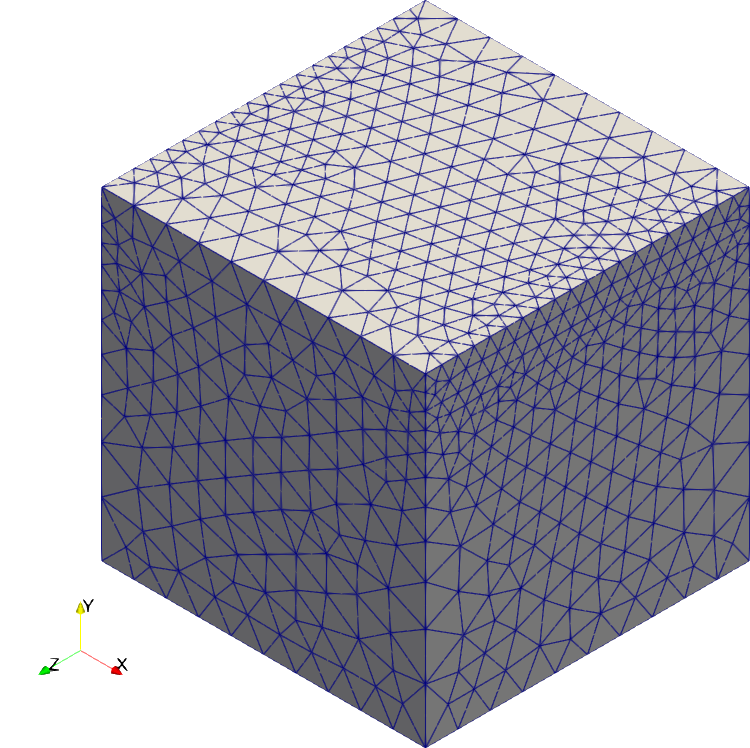
\includegraphics[width=\linewidth]{Figuras/FSI-Cavity3D/fluid-mesh.png}
        \caption{Fluido - malha m1.}
    \end{subfigure}
    \begin{subfigure}[b]{0.4\textwidth}
        \centering
        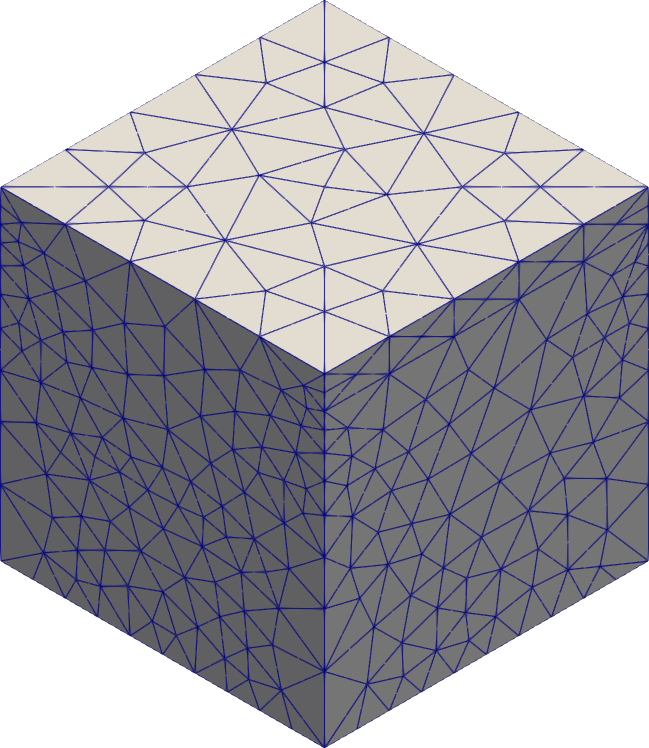
\includegraphics[width=.85\linewidth]{Figuras/FSI-Cavity3D/fm2.png}
        \caption{Fluido - malha m2.}
    \end{subfigure}
    \begin{subfigure}[b]{0.4\textwidth}
        \centering
        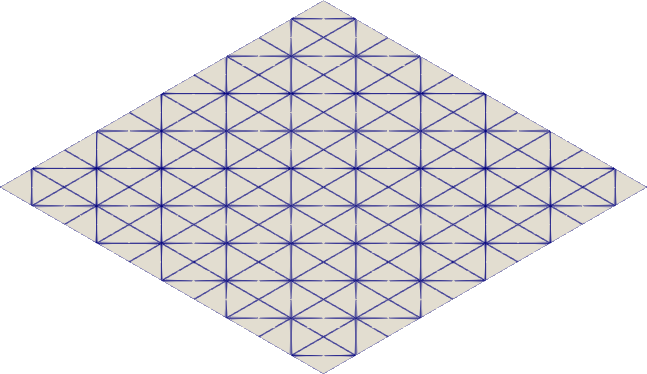
\includegraphics[width=\linewidth]{Figuras/FSI-Cavity3D/shell-mesh.png}
        \caption{Casca.}
    \end{subfigure}
    \\Fonte: Presente trabalho (\the\year).
    \label{fig:Cavity3D-mesh}
\end{figure}

Observou-se a influência que cada tipo de estabilização causa na solução, onde simulou-se com as estabilizações SUPG/PSPG e VMS para a malha m2, enquanto a malha m1 foi estabilizada por SUPG/PSPG como referência. Também foram simulados os problemas com e sem a aplicação do modelo LES, para analisar os efeitos que este causa na solução. A Figura \ref{fig:Cavity3D-rescoarse} apresenta o deslocamento vertical do centro da casca ao longo do tempo, comparando-se com os resultados obtidos por \citeonline{valdes2007nonlinear} e por \citeonline{fernandes2016interaccao} e com a simulação com malha mais fina.

\begin{figure}[h!]
    \centering
    \caption{Cavidade tridimensional - Deslocamento vertical do centro da casca ao longo do tempo para o segundo caso.}
    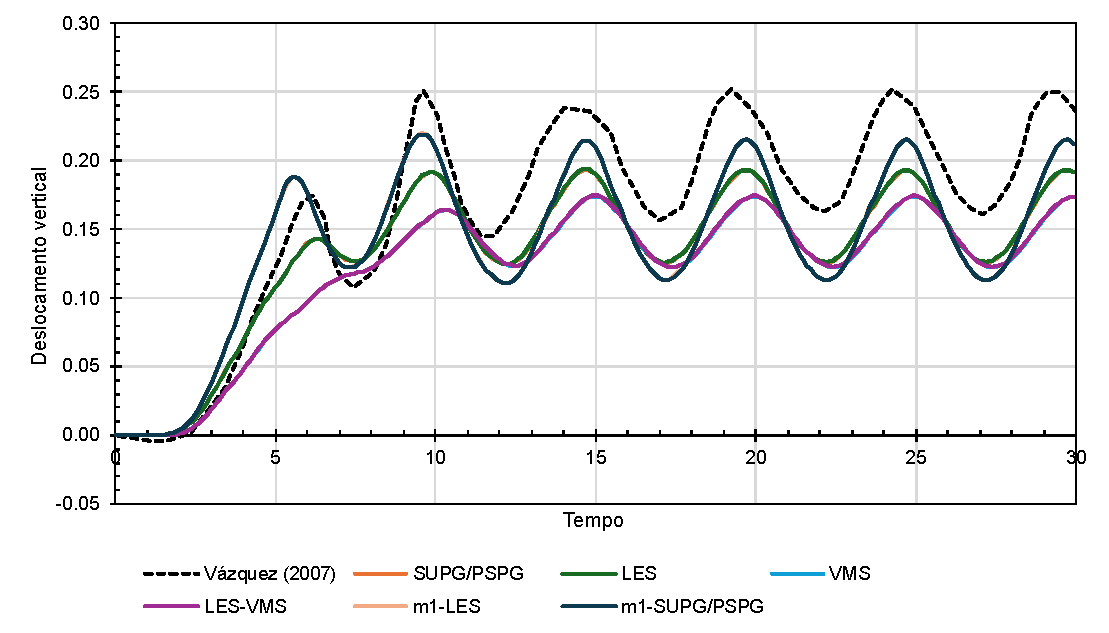
\includegraphics[width=\linewidth]{Figuras/FSI-Cavity3D/FSI-cavity3D.pdf}
    \\Fonte: Presente trabalho (\the\year)
    \\\small{Nota: A linha referente à simulação LES sobrepõe a de SUPG/PSPG; e a linha referente à LES-VMS sobrepõe a VMS.}
    \label{fig:Cavity3D-rescoarse}
\end{figure}

Verifica-se que a aplicação dos demais termos estabilizadores presentes na formulação VMS levaram a uma solução mais amortecida em relação ao SUPG/PSPG. No entanto, a aplicação do modelo LES não surtiu efeito na solução encontrada, o que se deve ao fato do número de Reynolds do problema ser baixo, além de possuir gradientes de velocidade também muito pequenos.

A Figura \ref{fig:Cavity3D-time} apresenta a distribuição de deslocamentos verticais sobre a casca deformada nos instantes $t=4,0$, $6,0$, $21,8$ e $24,3$ para a simulação empregando a malha m1, os quais são bem próximos aos obtidos por \citeonline{valdes2007nonlinear}. A figura \ref{fig:Cavity3D-press} apresenta o campo de pressão e de velocidade para os mesmos instantes de tempo.

\begin{figure}[h!]
    \centering
    \caption{Cavidade tridimensional - Deslocamento vertical da casca.}
    \begin{subfigure}[b]{0.35\textwidth}
        \centering
        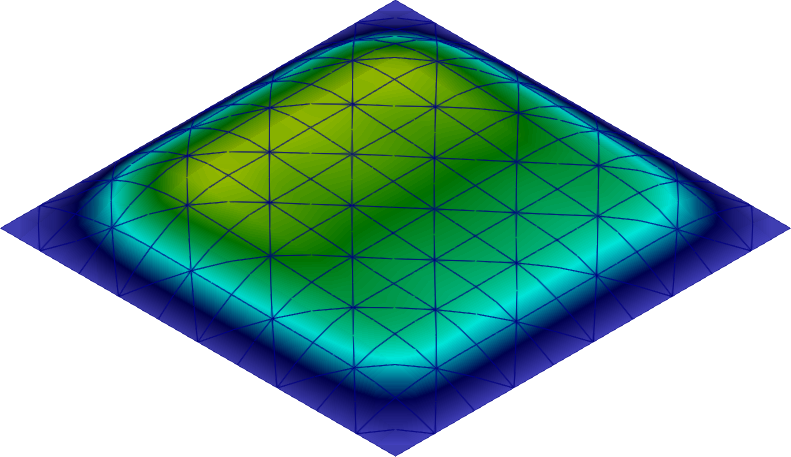
\includegraphics[width=.9\linewidth]{Figuras/FSI-Cavity3D/d4.png}
        \caption{$t=4,0$}
    \end{subfigure}
    \begin{subfigure}[b]{0.35\textwidth}
        \centering
        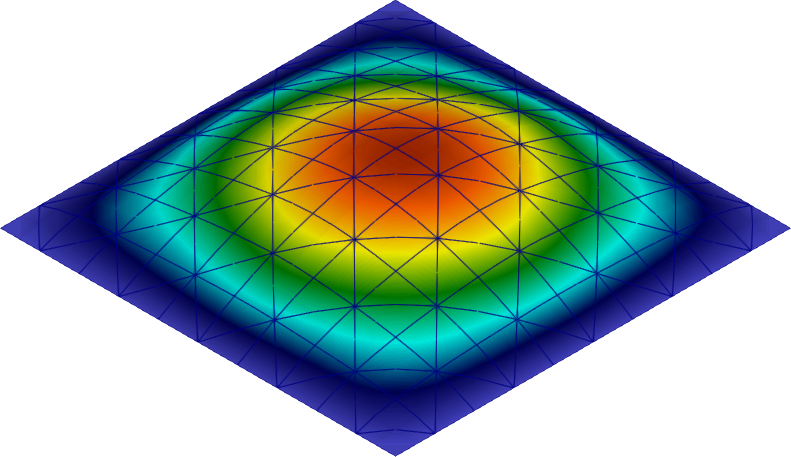
\includegraphics[width=.9\linewidth]{Figuras/FSI-Cavity3D/d6.png}
        \caption{$t=6,0$}
    \end{subfigure}\\
    \begin{subfigure}[b]{0.35\textwidth}
        \centering
        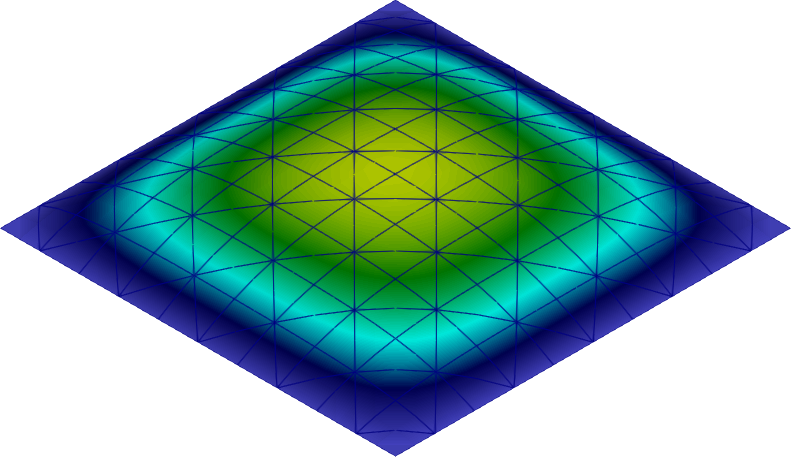
\includegraphics[width=.9\linewidth]{Figuras/FSI-Cavity3D/d21-8.png}
        \caption{$t=21,8$}
    \end{subfigure}
    \begin{subfigure}[b]{0.35\textwidth}
        \centering
        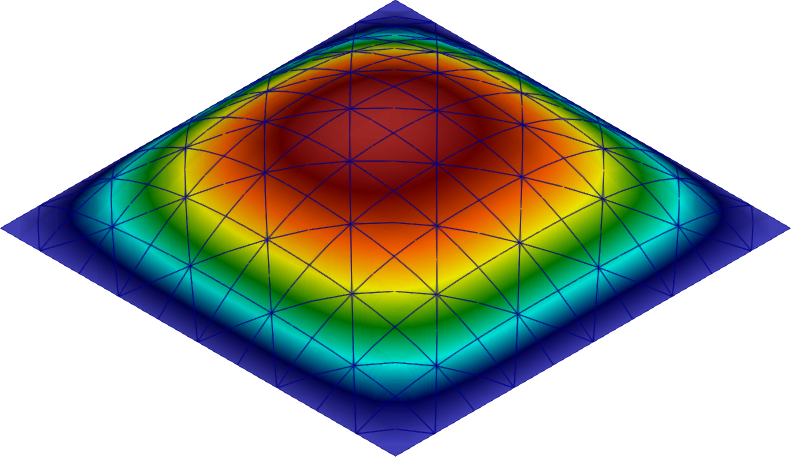
\includegraphics[width=.9\linewidth]{Figuras/FSI-Cavity3D/d24-3.png}
        \caption{$t=24,3$}
    \end{subfigure}
    \begin{subfigure}[b]{0.5\textwidth}
        \centering
        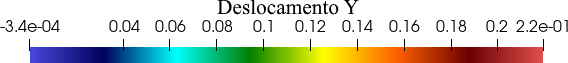
\includegraphics[width=\linewidth]{Figuras/FSI-Cavity3D/ld.png}
    \end{subfigure}
    \\Fonte: Presente trabalho (\the\year).
    \label{fig:Cavity3D-time}
\end{figure}

\begin{figure}[h!]
    \centering
    \caption{Cavidade tridimensional - Campo de pressão e de velocidade na cavidade.}
    \begin{subfigure}[b]{0.23\textwidth}
        \caption*{Campo de pressão}
        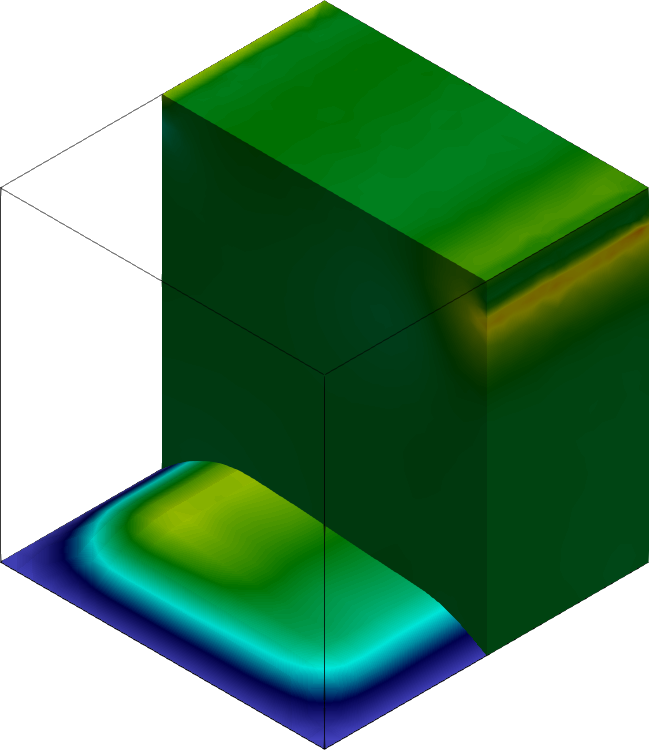
\includegraphics[width=\linewidth]{Figuras/FSI-Cavity3D/p4.png}
    \end{subfigure}
    \begin{subfigure}[b]{0.23\textwidth}
        \caption*{Campo de velocidade}
        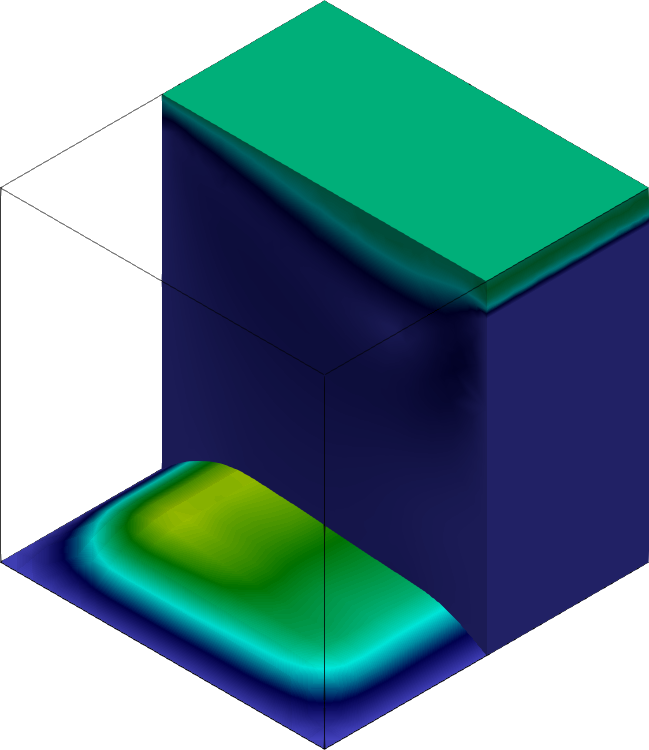
\includegraphics[width=\linewidth]{Figuras/FSI-Cavity3D/u4.png}
    \end{subfigure}
    \caption*{$t=4,0$}
    \begin{subfigure}[b]{0.23\textwidth}
        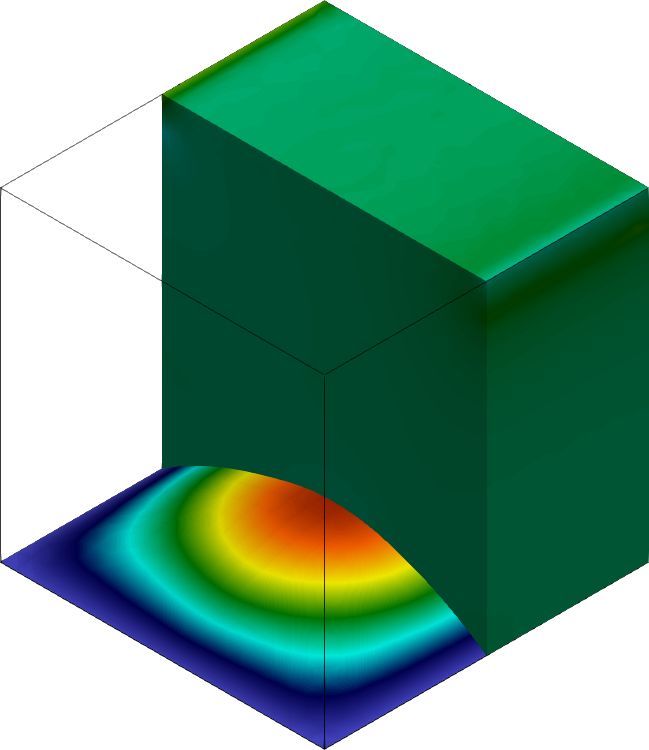
\includegraphics[width=\linewidth]{Figuras/FSI-Cavity3D/p6.png}
    \end{subfigure}
    \begin{subfigure}[b]{0.23\textwidth}
        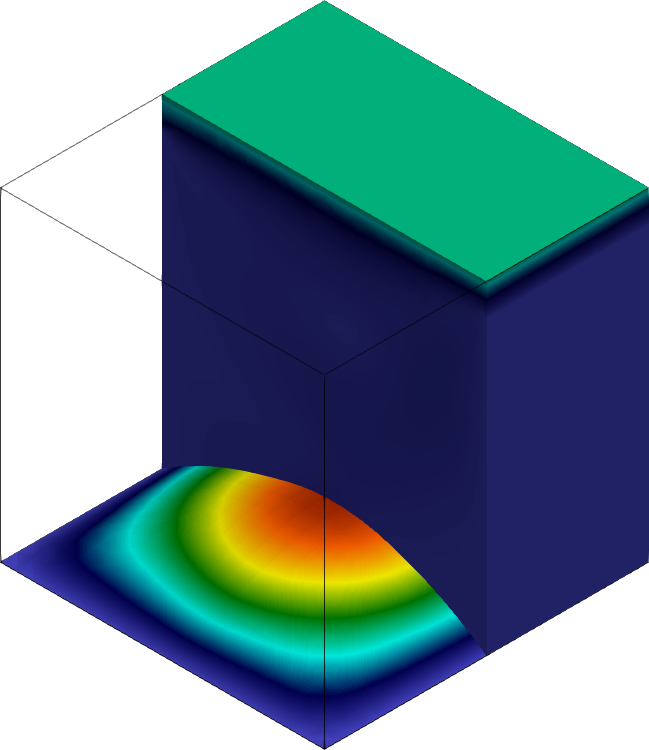
\includegraphics[width=\linewidth]{Figuras/FSI-Cavity3D/u6.png}
    \end{subfigure}
    \caption*{$t=6,0$}
    \begin{subfigure}[b]{0.23\textwidth}
        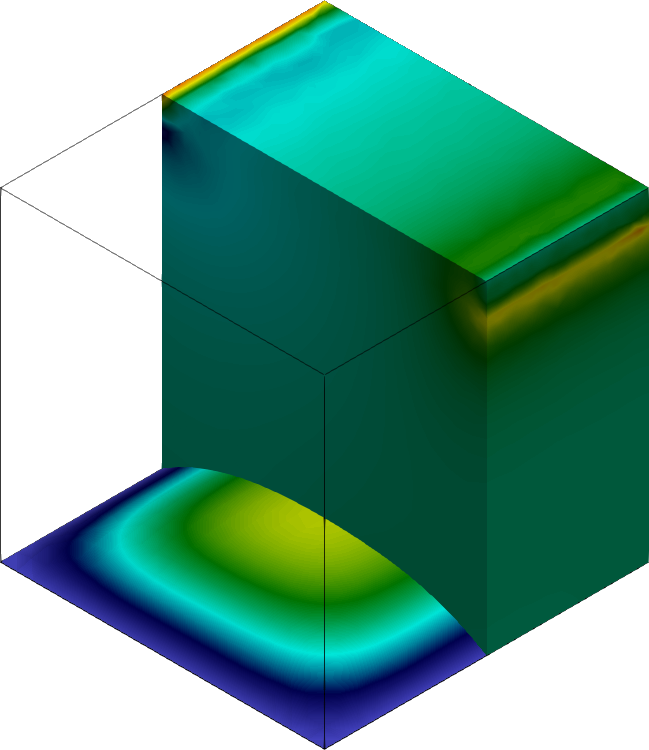
\includegraphics[width=\linewidth]{Figuras/FSI-Cavity3D/p21-8.png}
    \end{subfigure}
    \begin{subfigure}[b]{0.23\textwidth}
        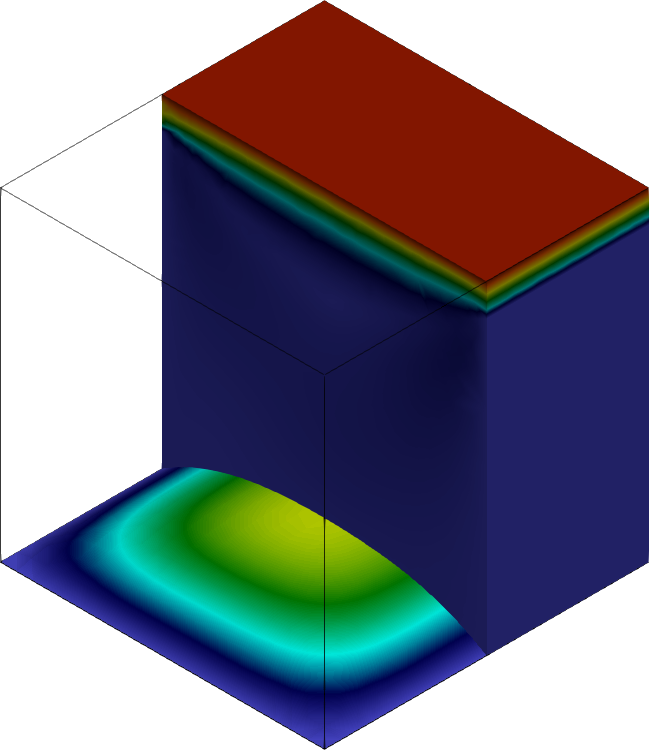
\includegraphics[width=\linewidth]{Figuras/FSI-Cavity3D/u21-8.png}
    \end{subfigure}
    \caption*{$t=21,8$}
    \begin{subfigure}[b]{0.23\textwidth}
        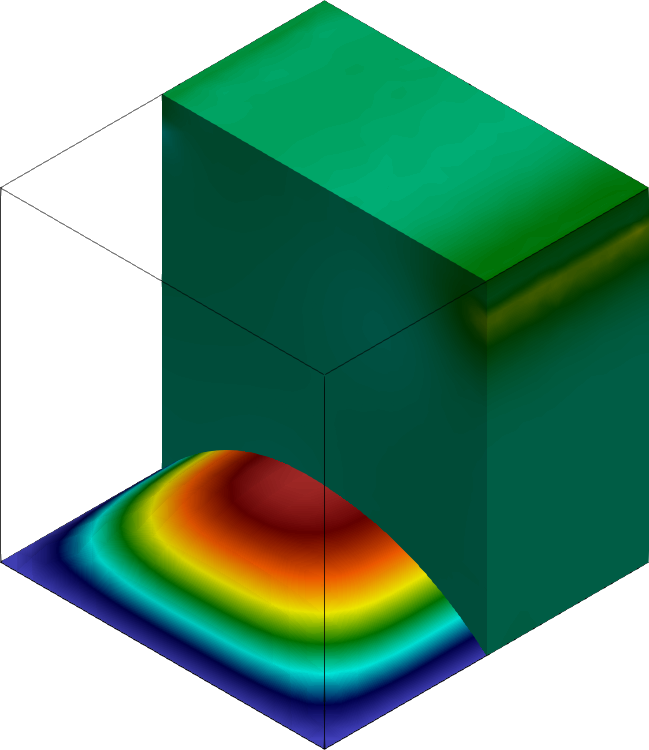
\includegraphics[width=\linewidth]{Figuras/FSI-Cavity3D/p24-3.png}
    \end{subfigure}
    \begin{subfigure}[b]{0.23\textwidth}
        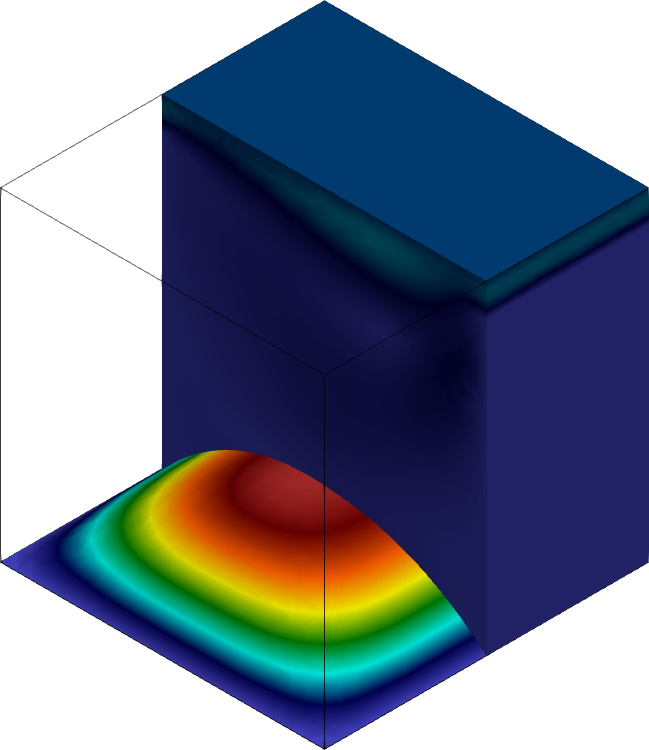
\includegraphics[width=\linewidth]{Figuras/FSI-Cavity3D/u24-3.png}
    \end{subfigure}
    \caption*{$t=24,3$}
    \begin{subfigure}[b]{0.35\textwidth}
        
\includegraphics[width=\linewidth]{Figuras/FSI-Cavity3D/lp.png}
    \end{subfigure}
    \begin{subfigure}[b]{0.35\textwidth}
        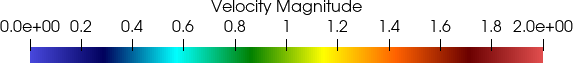
\includegraphics[width=\linewidth]{Figuras/FSI-Cavity3D/lu.png}
    \end{subfigure}
    \\Fonte: Presente trabalho (\the\year).
    \label{fig:Cavity3D-press}
\end{figure}

\newpage
%==================================================================================================
\subsection{\textit{Flutter} em painel flexível} \label{FSI-prism}
%==================================================================================================

Outro problema comumente simulado para a verificação de formulações para análise de interação fluido-estrutura, proposto por \citeonline{wall1998fluid}, trata-se de um painel engastado a um prisma quadrado rígido, como observado na Figura \ref{fig:FSI-prism}. Tal problema possui comportamento fortemente acoplado, além de apresentar certa complexidade, uma vez que o desprendimento de vórtices ocasionado pelo escoamento em torno do prisma que gera perturbações no escoamento de forma a induzir vibrações na estrutura, chegando a grandes deslocamentos.

O painel possui comprimento $L=4$ cm e espessura $h_0=0,06$ cm, sendo engastado em um bloco rígido de dimensões $1\times 1$ cm², sua massa específica é $\rho_S=0,1$ g/cm³ e seu módulo de Young $E=2,5\times 10^6$ g/(cm$\cdot$s²). O coeficiente de Poisson desse problema foi considerado nulo, de forma a representar melhor a solução da referência que emprega simulação bidimensional com elementos de biga de  Euler-Bernoulli. O fluido que envolve a estrutura possui massa específica $\rho_f=1,18\times10^{-3}$ g/cm³ e viscosidade dinâmica $\mu=1,82\times10^{-4}$ g/(cm$\cdot$s), modelado em um domínio $\Omega=[0,21]\times[0,12]$ cm², com uma velocidade de entrada constante $u_\infty=51,3$ cm/s na direção 1, o que resulta em um número de Reynolds de $333$, ao considerar o comprimento característico o lado do prisma. Esse problema é conhecido pelo comportamento bidimensional das variáveis envolvidas, no entanto a simulação foi realizada considerando um problema tridimensional, assim foi considerada uma espessura $esp=0,1$ cm para o domínio computacional, assim como imposição de deslocamento nulo do painel na terceira direção e do travamento dessa componente no vetor generalizado, enquanto no fluido foi considerada uma condição de simetria nas faces frontal e traseira do domínio.

\begin{figure}[h!]
    \centering
    \caption{\textit{Flutter} em painel - Desenho esquemático do problema.}
    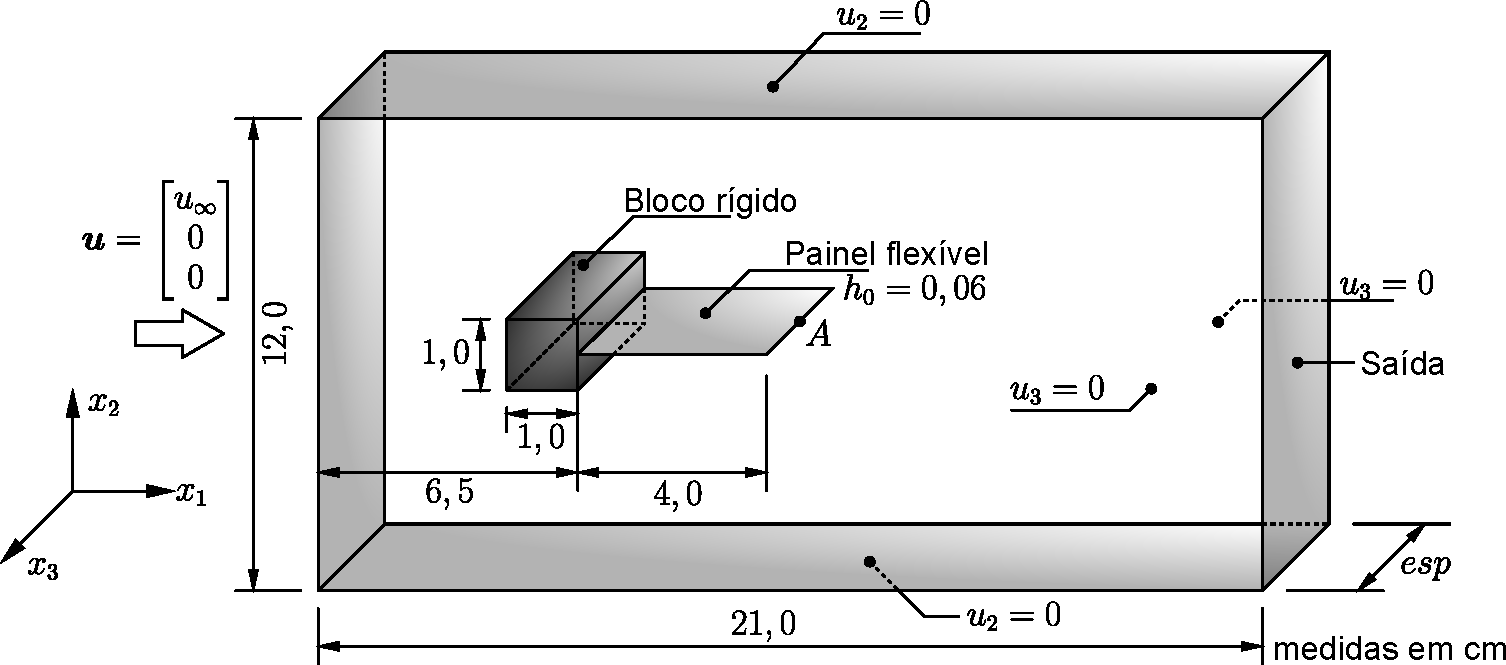
\includegraphics[width=\linewidth]{Figuras/FSI-prism/FSI-prism3D.pdf}
    \\Fonte: Presente trabalho (\the\year).
    \label{fig:FSI-prism}
\end{figure}

% Segundo \citeonline{WARBURTON1976109}, o qual considera uma teoria clássica da dinâmica das estruturas, tem-se que os três primeiros modos de vibração de uma viga engastada com essas dimensões são $f_1=0,606$ Hz, $f_2=3,796$ Hz e $f_3=10,630$ Hz. Já a frequência de desprendimento de vórtices pode ser obtida ao manter toda a estrutura rígida, que segundo \citeonline{hubner2004monolithic}, resulta em $f_v=3,7$ Hz, o que se aproxima do segundo modo de vibração da estrutura, levando, portanto, à dominância desse modo.

O domínio computacional do fluido foi discretizado em 3423 elementos tetraédricos de aproximação quadrática, possuindo 7088 nós e 28352 graus de liberdade. Já o domínio computacional da casca foi discretizado em 54 elementos e 165 nós, resultando em 1155 graus de liberdade. A Figura \ref{fig:meshPanel} apresenta as malhas utilizadas em ambos os domínios. O intervalo de tempo analisado foi $t\in[0,5]$, discretizado em passos de tempo $\Delta t=1,65\times10^{-3}$. O esquema de integração temporal foi dado considerando um raio espectral $\rho_\infty=0,0$ e os termos estabilizadores adotados foram da formulação SUPG/PSPG.

\begin{figure}[h!]
    \centering
    \caption{\textit{Flutter} em painel - Malha utilizada para os domínios da simulação de painel.}
    \begin{subfigure}[b]{\textwidth}
        \centering
        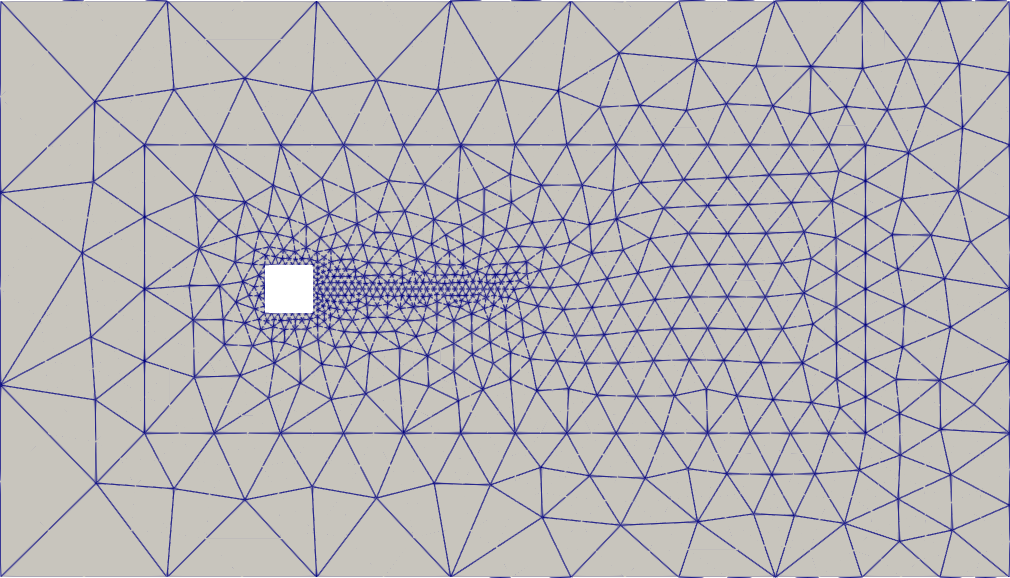
\includegraphics[width=.8\linewidth]{Figuras/FSI-prism/meshFluid.png}
        \caption{Malha do fluido.}
    \end{subfigure}
    \begin{subfigure}[b]{\textwidth}
        \centering
        
\includegraphics[width=.8\linewidth]{Figuras/FSI-prism/meshSolid.png}
        \caption{Malha da casca.}
    \end{subfigure}
    \\Fonte: Presente trabalho (\the\year).
    \label{fig:meshPanel}
\end{figure}

O gráfico apresentado na Figura \ref{fig:prismRes} indica o deslocamento vertical da extremidade do painel ao longo do tempo em comparação com os resultados obtidos por \citeonline{wall1999fluid}.

\begin{figure}[h!]
    \centering
    \caption{\textit{Flutter} em painel - Deslocamento vertical na extremidade do painel ao longo do tempo.}
    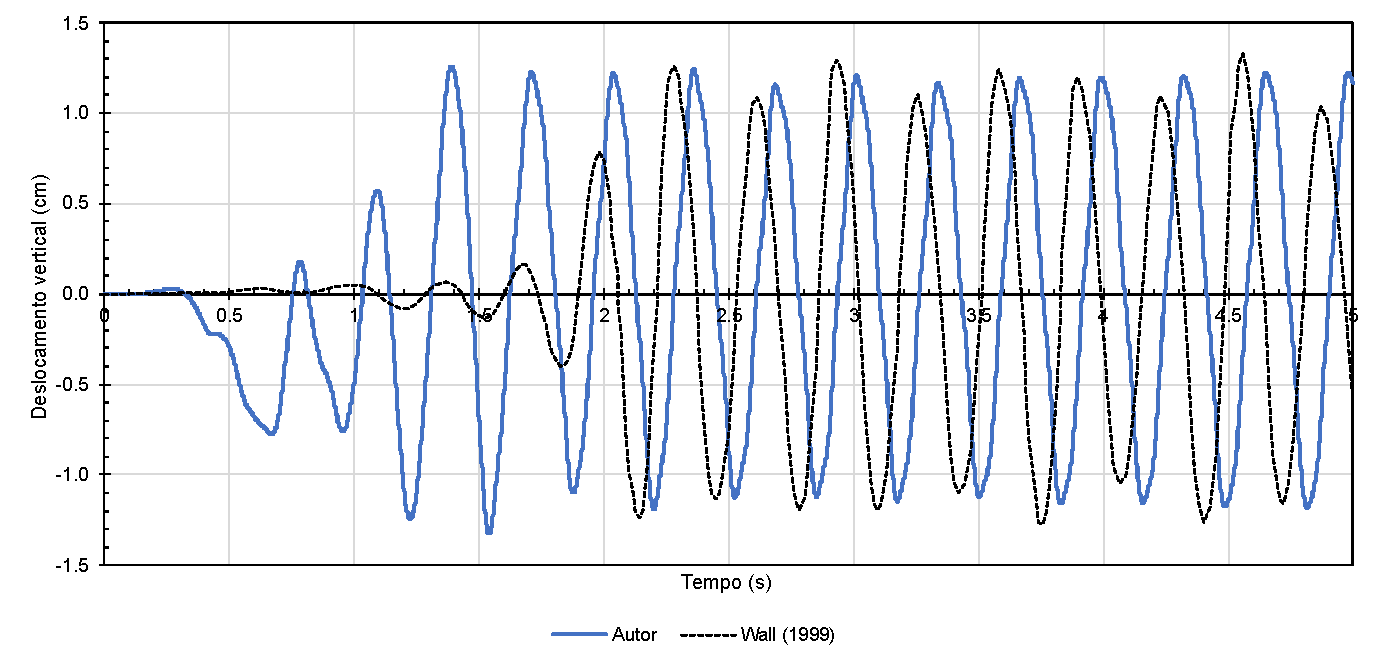
\includegraphics[width=\linewidth]{Figuras/FSI-prism2/results.pdf}
    \\Fonte: Presente trabalho (\the\year).
    \label{fig:prismRes}
\end{figure}

Assim, obteve-se um comportamento oscilatório com amplitude de 1,26 cm e frequência de 3,03 Hz (Período de 0,33 s), o que se aproxima dos resultados de \citeonline{wall1999fluid}.

As Figuras \ref{fig:prismVel2} a \ref{fig:prismMesh2} apresentam os campos de velocidade, pressões e a configuração da malha para frações $T/6$ do período, respectivamente.

\begin{figure}[h!]
    \centering
    \caption{\textit{Flutter} em painel - Magnitude do campo de velocidade.}
    \begin{subfigure}[b]{0.32\textwidth}
        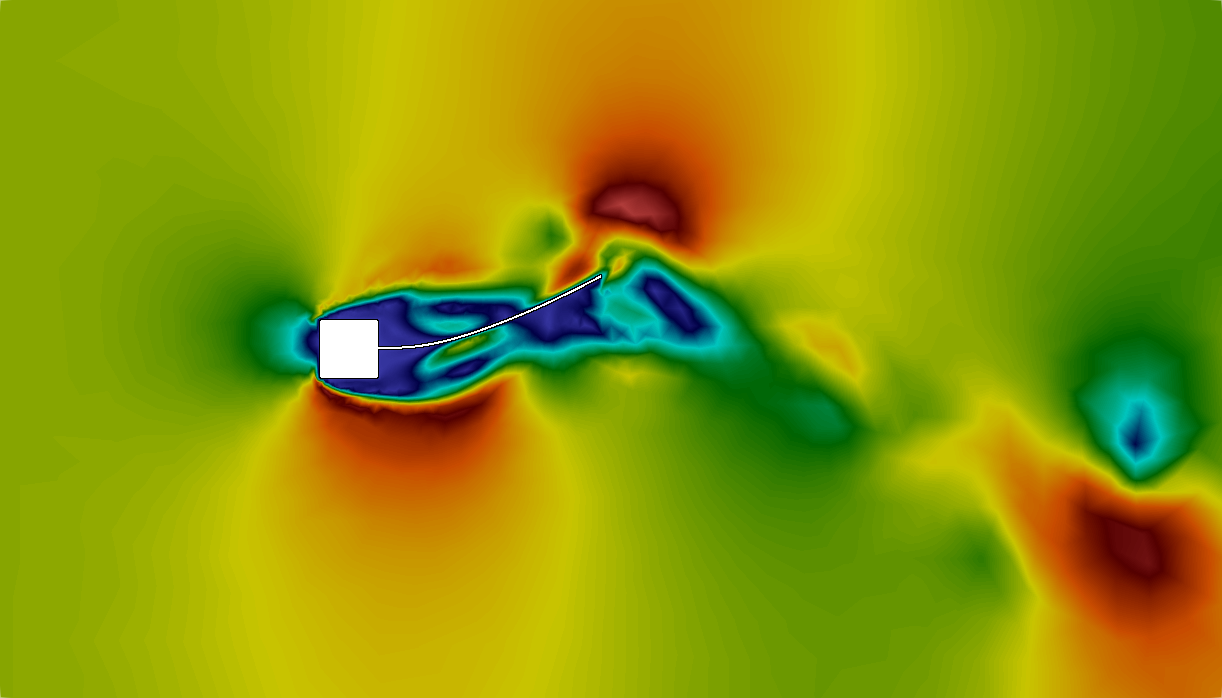
\includegraphics[width=\linewidth]{Figuras/FSI-prism2/vT1.png}
        \caption{$t=nT$}
    \end{subfigure}
    \begin{subfigure}[b]{0.32\textwidth}
        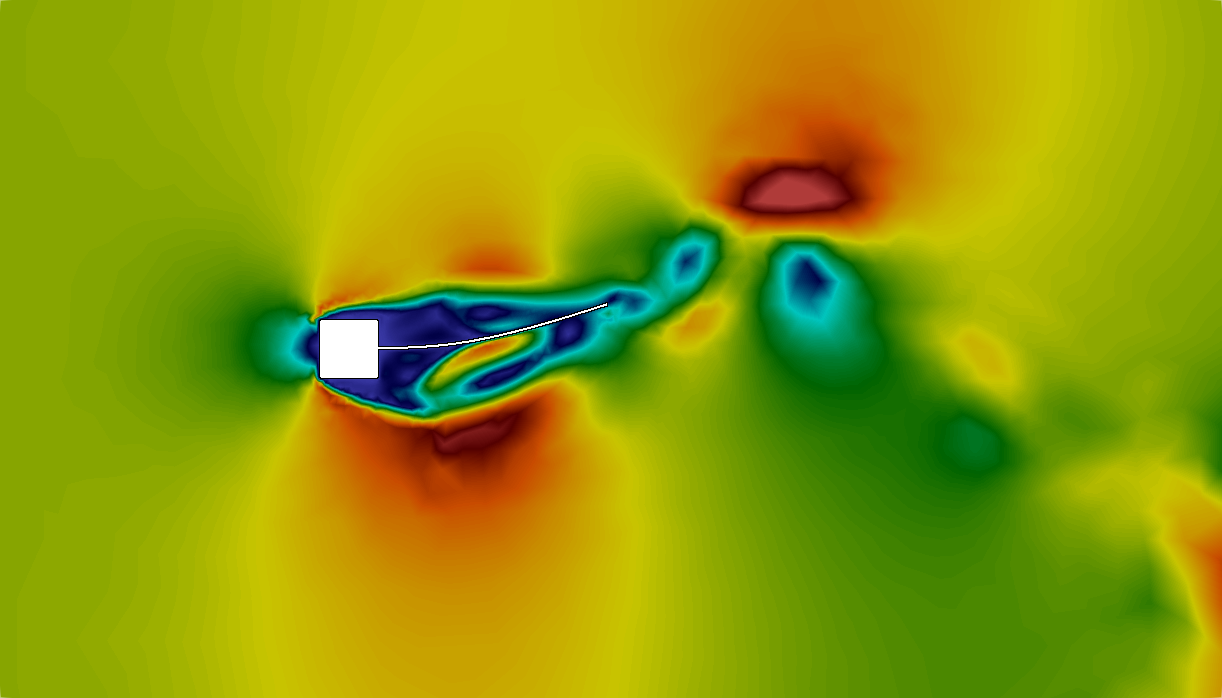
\includegraphics[width=\linewidth]{Figuras/FSI-prism2/vT2.png}
        \caption{$t=nT+T/6$}
    \end{subfigure}
    \begin{subfigure}[b]{0.32\textwidth}
        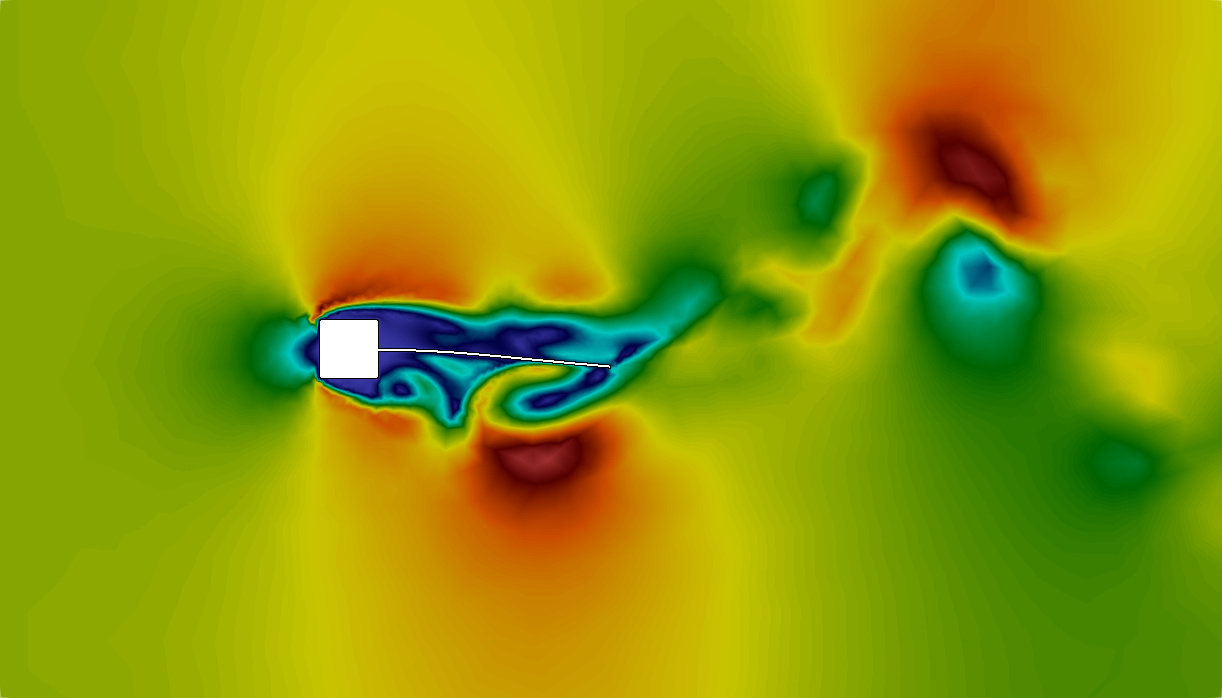
\includegraphics[width=\linewidth]{Figuras/FSI-prism2/vT3.png}
        \caption{$t=nT+2T/6$}
    \end{subfigure}
    \begin{subfigure}[b]{0.32\textwidth}
        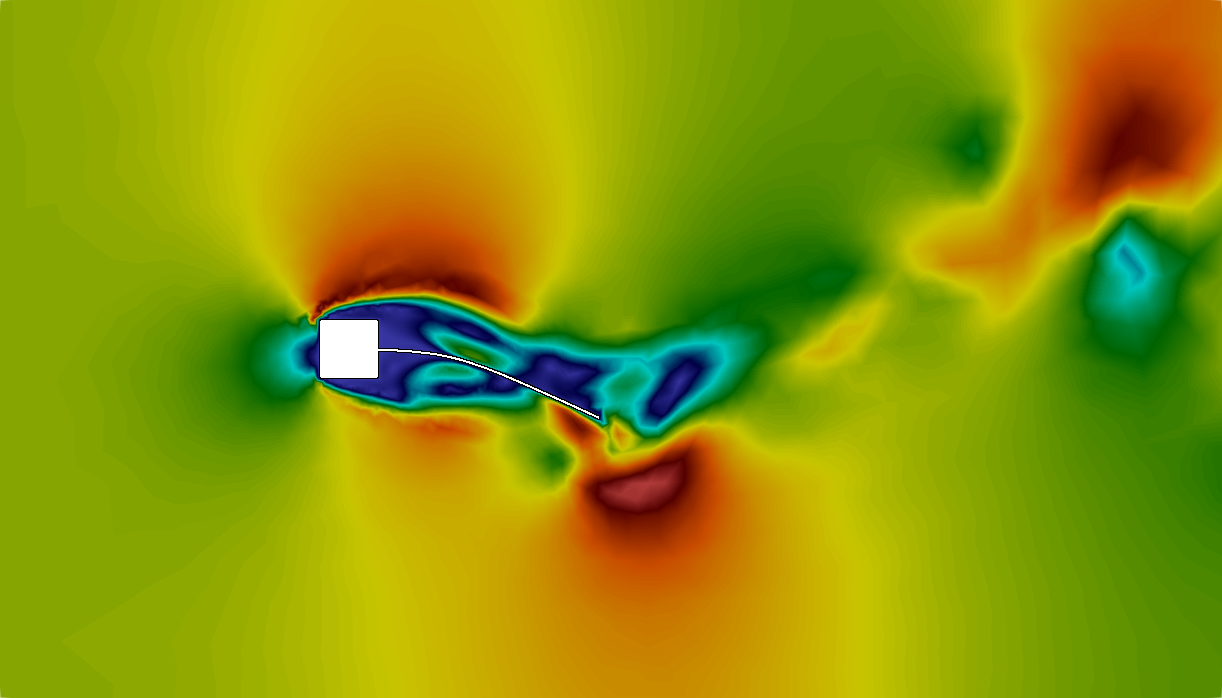
\includegraphics[width=\linewidth]{Figuras/FSI-prism2/vT4.png}
        \caption{$t=nT+3T/6$}
    \end{subfigure}
    \begin{subfigure}[b]{0.32\textwidth}
        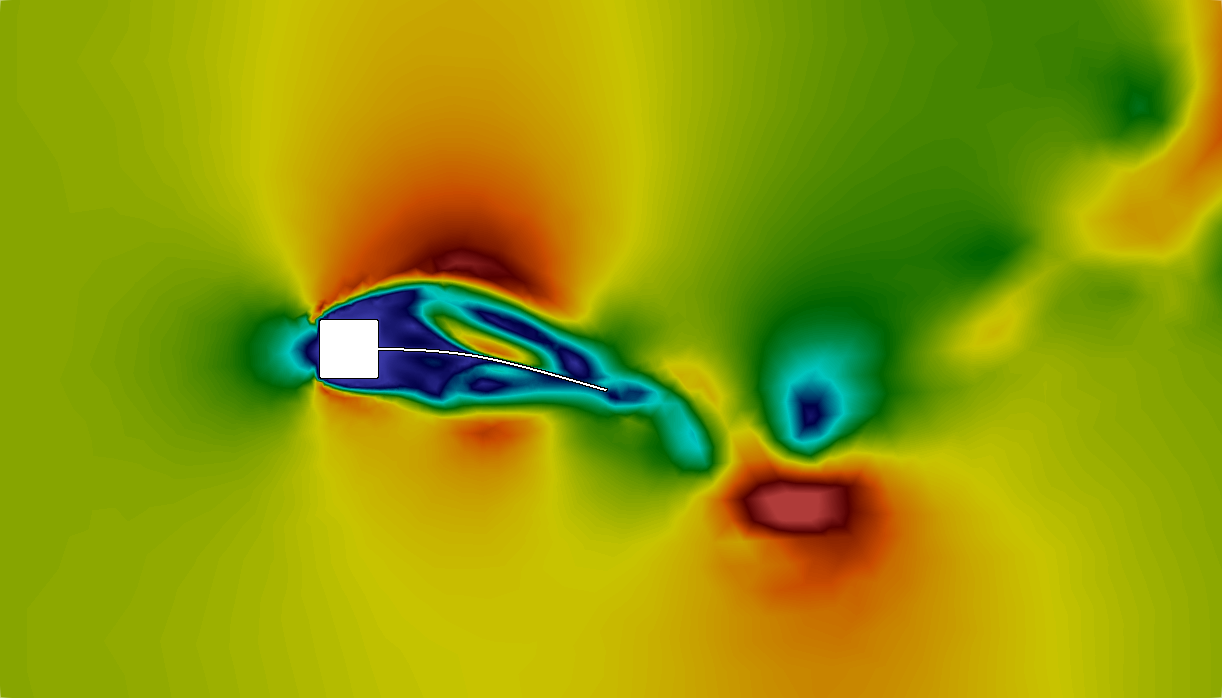
\includegraphics[width=\linewidth]{Figuras/FSI-prism2/vT5.png}
        \caption{$t=nT+4T/6$}
    \end{subfigure}
    \begin{subfigure}[b]{0.32\textwidth}
        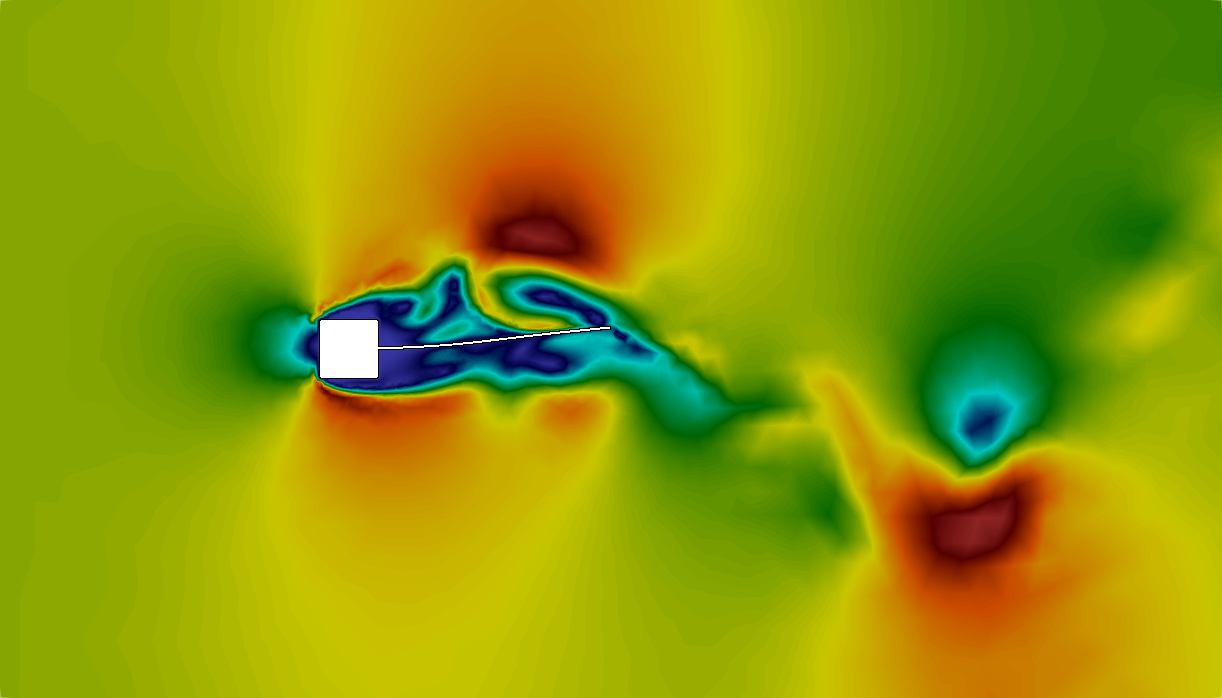
\includegraphics[width=\linewidth]{Figuras/FSI-prism2/vT6.png}
        \caption{$t=nT+5T/6$}
    \end{subfigure}
    \begin{subfigure}[b]{0.49\textwidth}
        
\includegraphics[width=\linewidth]{Figuras/FSI-prism2/vLegenda.png}
    \end{subfigure}
    \\Fonte: Presente trabalho (\the\year).
    \label{fig:prismVel2}
\end{figure}

\begin{figure}[h!]
    \centering
    \caption{\textit{Flutter} em painel - Campo de pressão.}
    \begin{subfigure}[b]{0.32\textwidth}
        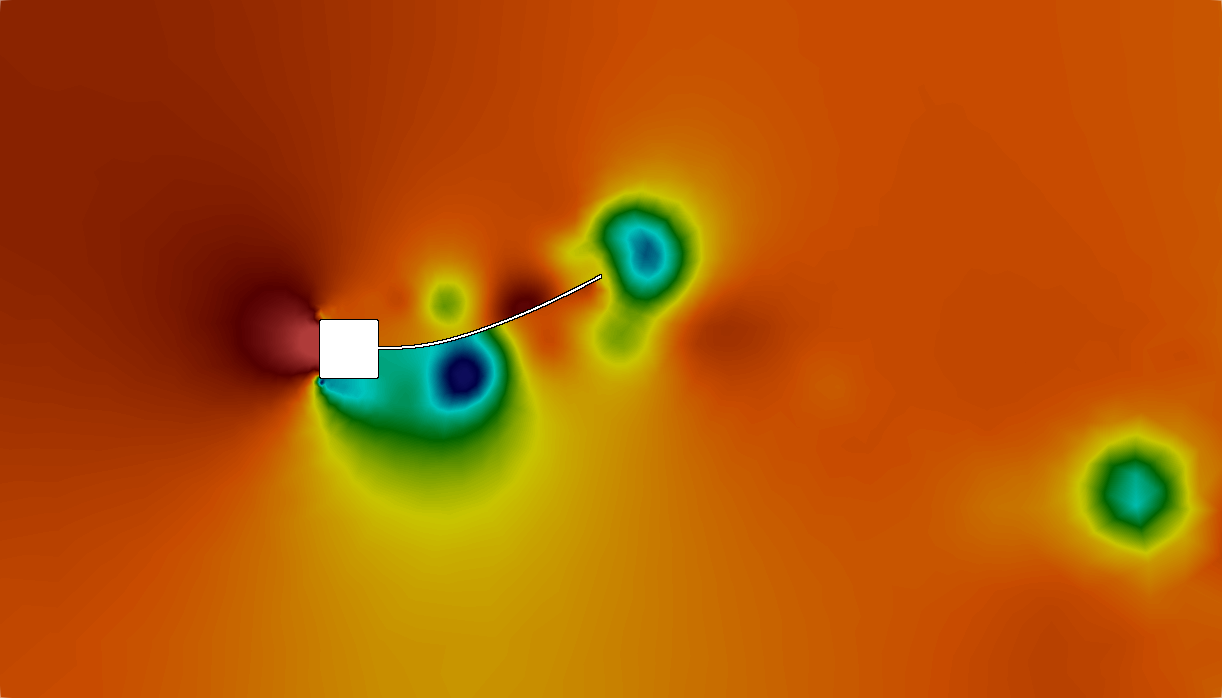
\includegraphics[width=\linewidth]{Figuras/FSI-prism2/pT1.png}
        \caption{$t=nT$}
    \end{subfigure}
    \begin{subfigure}[b]{0.32\textwidth}
        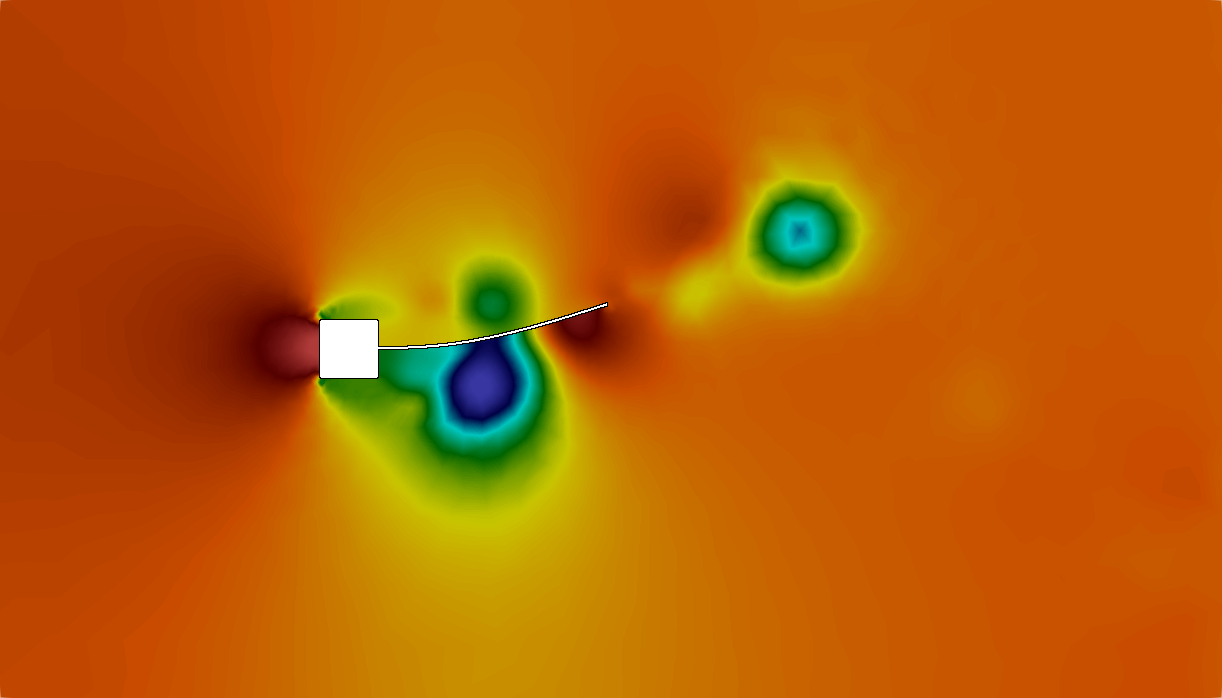
\includegraphics[width=\linewidth]{Figuras/FSI-prism2/pT2.png}
        \caption{$t=nT+T/6$}
    \end{subfigure}
    \begin{subfigure}[b]{0.32\textwidth}
        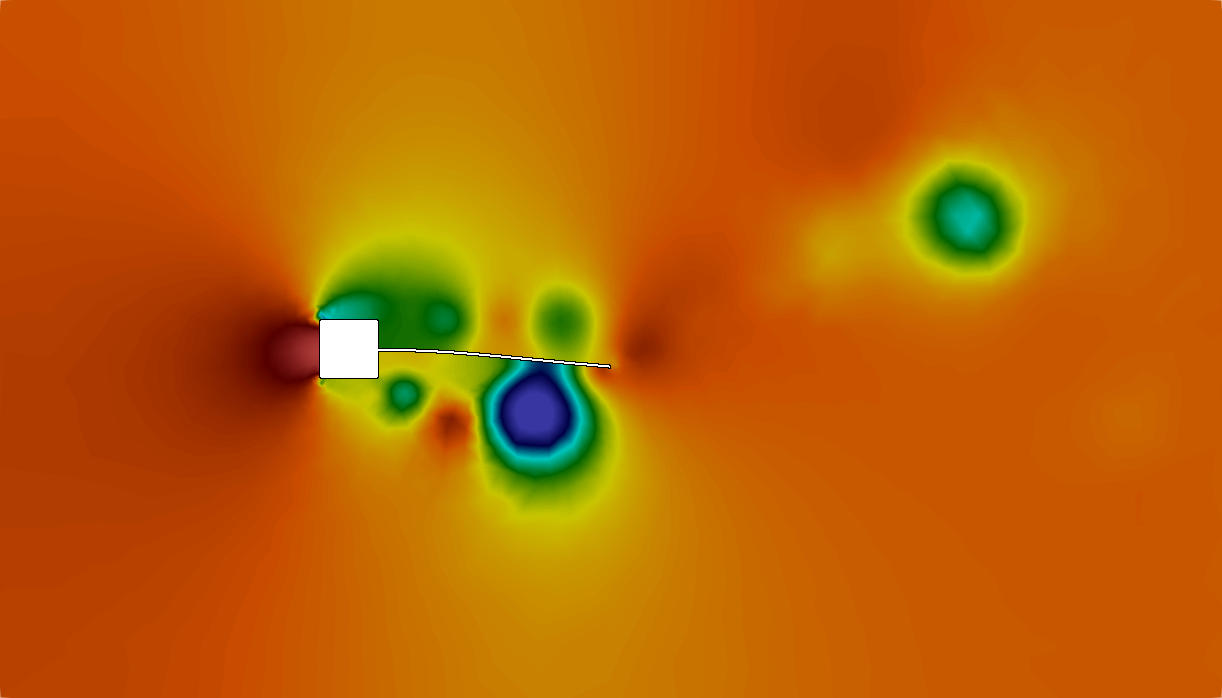
\includegraphics[width=\linewidth]{Figuras/FSI-prism2/pT3.png}
        \caption{$t=nT+2T/6$}
    \end{subfigure}
    \begin{subfigure}[b]{0.32\textwidth}
        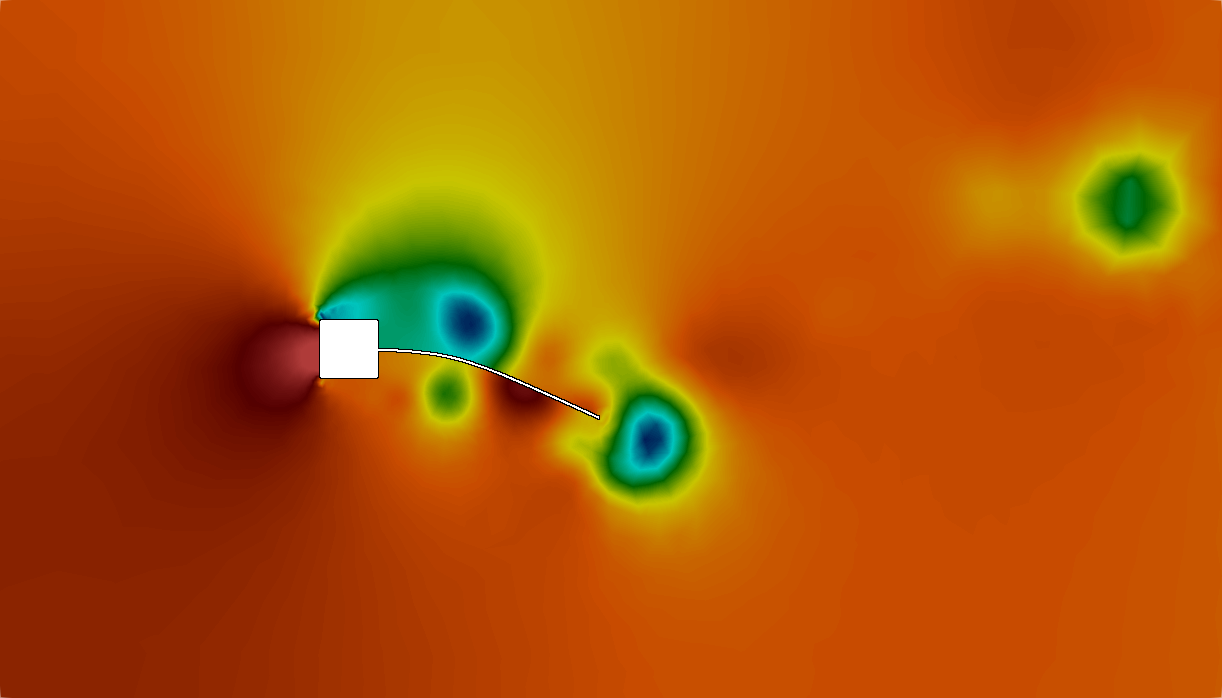
\includegraphics[width=\linewidth]{Figuras/FSI-prism2/pT4.png}
        \caption{$t=nT+3T/6$}
    \end{subfigure}
    \begin{subfigure}[b]{0.32\textwidth}
        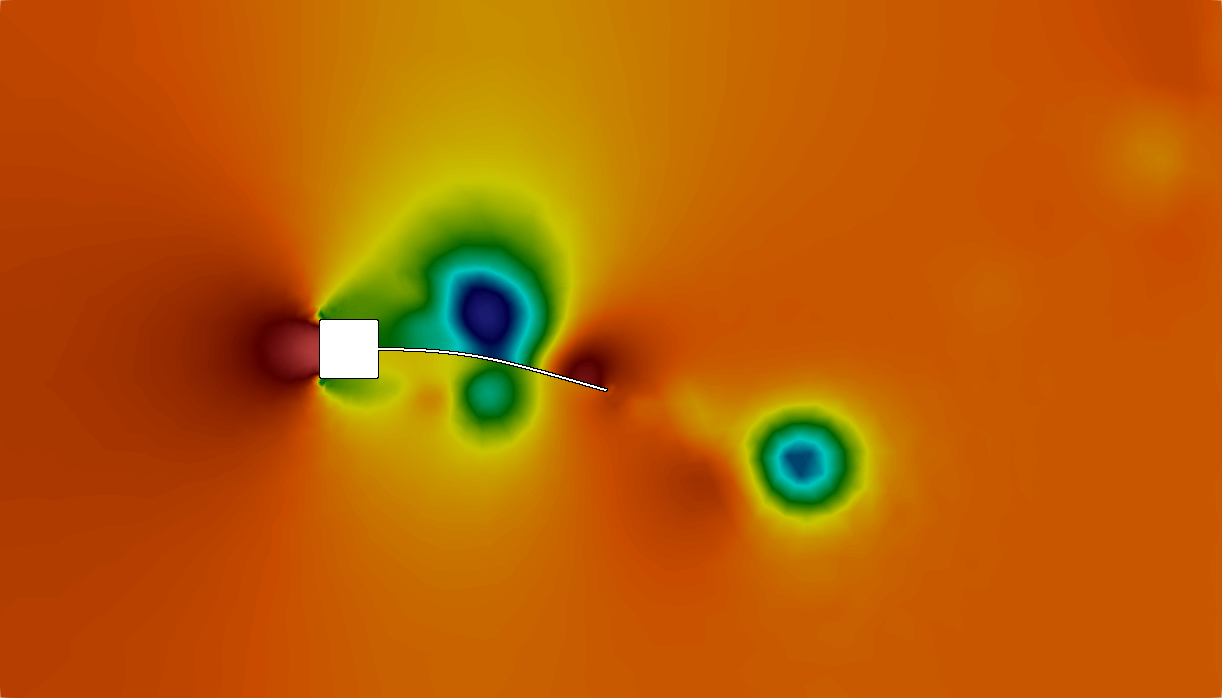
\includegraphics[width=\linewidth]{Figuras/FSI-prism2/pT5.png}
        \caption{$t=nT+4T/6$}
    \end{subfigure}
    \begin{subfigure}[b]{0.32\textwidth}
        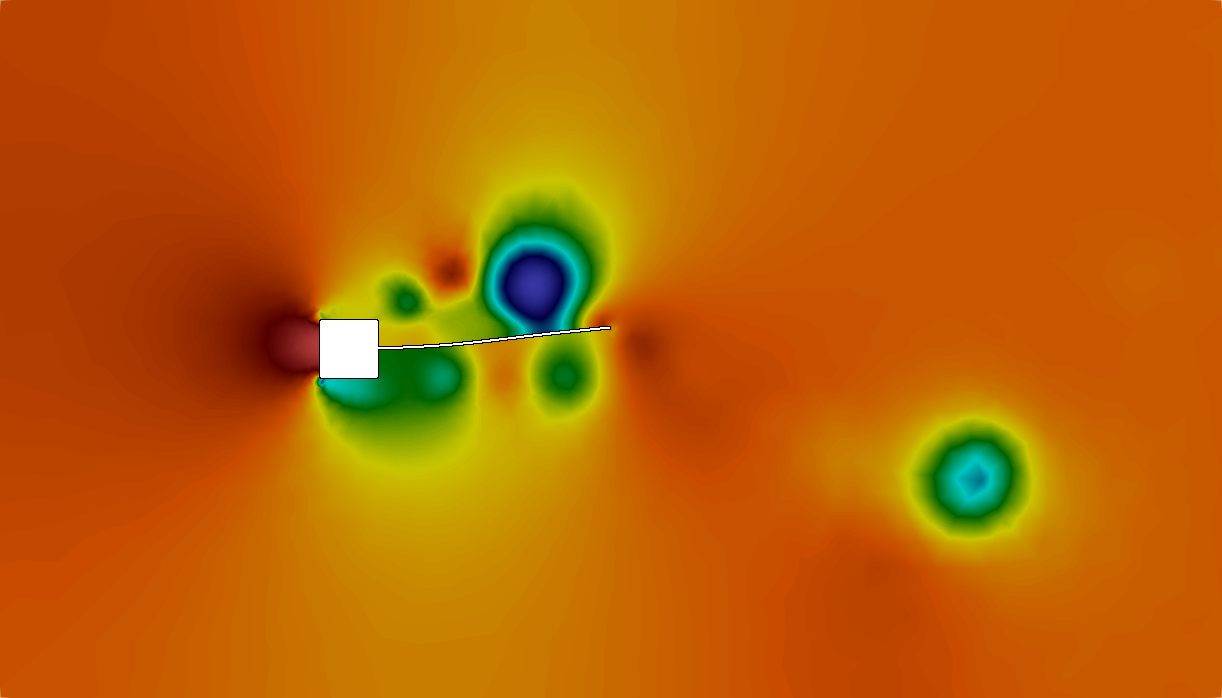
\includegraphics[width=\linewidth]{Figuras/FSI-prism2/pT6.png}
        \caption{$t=nT+5T/6$}
    \end{subfigure}
    \begin{subfigure}[b]{0.49\textwidth}
        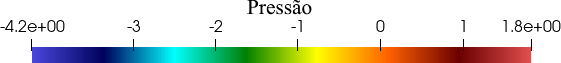
\includegraphics[width=\linewidth]{Figuras/FSI-prism2/pLegenda.png}
    \end{subfigure}
    \\Fonte: Presente trabalho (\the\year).
    \label{fig:prismPres2}
\end{figure}

\begin{figure}[h!]
    \centering
    \caption{\textit{Flutter} em painel - Configurações da malha.}
    \begin{subfigure}[b]{0.49\textwidth}
        \includegraphics[width=\linewidth]{Figuras/FSI-prism2/mT1.png}
        \caption{$t=nT$}
    \end{subfigure}
    \begin{subfigure}[b]{0.49\textwidth}
        \includegraphics[width=\linewidth]{Figuras/FSI-prism2/mT2.png}
        \caption{$t=nT+T/6$}
    \end{subfigure}
    \begin{subfigure}[b]{0.49\textwidth}
        \includegraphics[width=\linewidth]{Figuras/FSI-prism2/mT3.png}
        \caption{$t=nT+2T/6$}
    \end{subfigure}
    \begin{subfigure}[b]{0.49\textwidth}
        \includegraphics[width=\linewidth]{Figuras/FSI-prism2/mT4.png}
        \caption{$t=nT+3T/6$}
    \end{subfigure}
    \begin{subfigure}[b]{0.49\textwidth}
        \includegraphics[width=\linewidth]{Figuras/FSI-prism2/mT5.png}
        \caption{$t=nT+4T/6$}
    \end{subfigure}
    \begin{subfigure}[b]{0.49\textwidth}
        \includegraphics[width=\linewidth]{Figuras/FSI-prism2/mT6.png}
        \caption{$t=nT+5T/6$}
    \end{subfigure}
    \\Fonte: Presente trabalho (\the\year).
    \label{fig:prismMesh2}
\end{figure}
\newpage

Na sequência estudou-se o comportamento do painel quando modelado por uma malha pobre em um domínio de maior espessura. Assim, utilizou-se uma espessura $esp=4,0$, de forma que po painel possua uma geometria quadrada. Além disso também foi liberado o deslocamento do painel na terceira direção. Com isso, obtém-se uma malha de fluido contendo 6794 elementos quadráticos, com 11806 nós e 47224 graus de liberdade, enquanto a casca possui 200 elementos quadráticos, 441 nós e 3087 graus de liberdade. A Figura \ref{fig:meshPanel2} apresenta as malhas utilizadas em ambos os domínios.

\begin{figure}[h!]
    \centering
    \caption{\textit{Flutter} em painel - Malha pobre utilizada.}
    \begin{subfigure}[b]{0.49\textwidth}
        \includegraphics[width=\linewidth]{Figuras/flutter-coarse/fluid.png}
        \caption{Malha do fluido.}
    \end{subfigure}
    \begin{subfigure}[b]{0.49\textwidth}
        \includegraphics[width=\linewidth]{Figuras/flutter-coarse/shell.png}
        \caption{Malha da casca.}
    \end{subfigure}
    \\Fonte: Presente trabalho (\the\year).
    \label{fig:meshPanel2}
\end{figure}

O problema foi simulado com a aplicação das estabilizações SUPG/PSPG e VMS, com e sem aplicação do modelo LES. A Figura \ref{fig:prismRes2} apresenta o deslocamento vertical da extremidade do painel ao longo do tempo para as diferentes simulações em comparação com os resultados obtidos por \citeonline{wall1999fluid}. A Tabela \ref{tab:prismRes2} apresenta os valores de amplitude, período e frequência da oscilação após o problema atingir o equilíbrio dinâmico.

\begin{figure}[h!]
    \centering
    \caption{\textit{Flutter} em painel - Deslocamento vertical na extremidade para malha pobre.}
    \includegraphics[width=\linewidth]{Figuras/flutter-coarse/disp_y.pdf}
    \\Fonte: Presente trabalho (\the\year).
    \label{fig:prismRes2}
\end{figure}

\begin{table}[h!]
    \centering
    \caption{\textit{Flutter} em painel - Propriedades da oscilação para malha pobre.}
    \begin{tabular}{lccc}
        \hline
        Modelo        & Amplitude (cm) & Período (s) & Frequência (Hz) \\\hline
        SUPG/PSPG     & -              & -           & -               \\
        SUPG/PSPG+LES & 1,379          & 0,330       & 3,028           \\
        VMS           & 1,358          & 0,315       & 3,179           \\
        VMS+LES       & 1,384          & 0,327       & 3,062           \\\hline
    \end{tabular}
    \\Fonte: Presente trabalho (\the\year).
    \label{tab:prismRes2}
\end{table}

Verifica-se que o problema simulado com SUPG/PSPG não atingiu o equilíbrio dinâmico, com uma taxa de aumento da amplitude de deslocamento muito baixa. Já a simulação utilizando a mesma estabilização e o modelo LES já foi capaz de capturar corretamente o comportamento da estrutura. Por fim, tanto a simulação utilizando estabilização VMS, com e sem o LES, foi capaz de descrever adequadamente o comportamento da estrutura.